\chapter{Systematic Uncertainties}
\label{chap:syst}

The systematic uncertainty in the signal efficiency is estimated by estimating the systematic uncertainty of each efficiency factor in Eq.~\ref{eq:OverallEff}.

The systematic uncertainties in $\varepsilon_{\mathrm{track}}$, $\varepsilon_{\mathrm{vertexTrack}}$, and $\varepsilon_{\mathrm{vertexFit}}$ are studied using $K_{S}$ in Section~\ref{sec:syst:vertexing}. The systematic uncertainties in $\varepsilon_{\mathrm{trigger}}$ is studied in Section~\ref{sec:syst:trigger} using tag-and-probe method with $Z\rightarrow \ee,\mumu$ events. %The systematic uncertainties on $\varepsilon_{\mathrm{leptonID}}$ studied separately.


\section{Systematic Uncertainties in Tracking and Vertexing Efficiency}
\label{sec:syst:vertexing}

%\subsection{Data and MC comparison}
%\label{sec:vertexing_systematics_data_MC}
The systematic uncertainties in $\varepsilon_{\mathrm{track}}$, $\varepsilon_{\mathrm{vertexTrack}}$, and $\varepsilon_{\mathrm{vertexFit}}$ are estimated by comparing the tracking and vertexing efficiencies between the data and the background MC samples described in Section~\ref{sec:data_mc:data} using the process, $K_{S}\rightarrow\pi^{+}\pi^{-}$. In order to understand the validity and the limitation of this method, the kinematic distributions of $K_{S}$ and $Z'$ found in this method are compared in Appendix~\ref{app:syst_Ks_Zp}.

%In order to estimate the systematic uncertainties in reconstructing a displaced vertex, the tracking and vertexing efficiencies are compared between the data and the background MC samples described in Section~\ref{sec:data_sample} using $K_{S}\rightarrow\pi^{+}\pi^{-}$. % and its long lifetime ($c\tau \approx 26.84$ mm).

%The $K_{S}$ efficiency can be written as Eq.~\ref{eq:KaonEff}
%\begin{equation}
%\label{eq:KaonEff}
%\varepsilon_{K_{S}}=(\varepsilon_{\mathrm{track}}\cdot\varepsilon_{\mathrm{vertexTrack}})^2\cdot\varepsilon_{\mathrm{vertexFit}}=\bigg(\frac{N_{\mathrm{track}}}{N_{K_{S}}}\cdot\frac{N_{\mathrm{vertexTrack}}}{N_{\mathrm{track}}}\bigg)^2\cdot\frac{N_{\mathrm{vertex}}}{N_{\mathrm{trackPair}}}
%\end{equation}

Events are selected using the same event selection described in Section~\ref{sec:selection:pre}. %except trigger filter as electron or muon triggers are not useful for $K_{S}$ study. %In data sample, trigger applied?
From the selected events, $K_{S}$ candidates, referred as $K_{S}$ vertices, are selected by applying $K_{S}$ vertex selection to the secondary vertices in the events. $K_{S}$ vertex selection is similar to the $Z'$ signal vertex selection, but for the consistency with $K_{S}$ study in Run I and further background reduction, additional vertex cuts as described in Ref.~\cite{Aad:2011hd} are applied in $K_{S}$ vertex selection. The mass window of 0.35 to 0.65 GeV is used in the $K_{S}$ vertex selection. The difference between $K_{S}$ and $Z'$ vertex selections are summarized in Table~\ref{table:ks_vertex_cut}. Figure~\ref{fig:Ks_vertex_cutflow} shows $K_{S}$ vertex cut flow in the data and the background MC samples.

\begin{table}[!htb]
%\begin{table}[tb]
  \centering
  \begin{tabular}{ c c c }
    \hline
    \hline
    & $Z'$& $K_{S}$ \\
    \hline
    Vertex type & \mumu, \emu, \ee & \xx \\
    Mass (GeV) & $> 10.0$ & $[0.35,0.65]$ \\
    Additional cut & - & $K_{S}$ selection~\cite{Aad:2011hd} \\
    \hline
    \hline
  \end{tabular}
  \caption{Comparison of $Z'$ and $K_{S}$ vertex selections.}
  \label{table:ks_vertex_cut}
\end{table}

%\begin{figure}[tb]
\begin{figure}[!htb]
	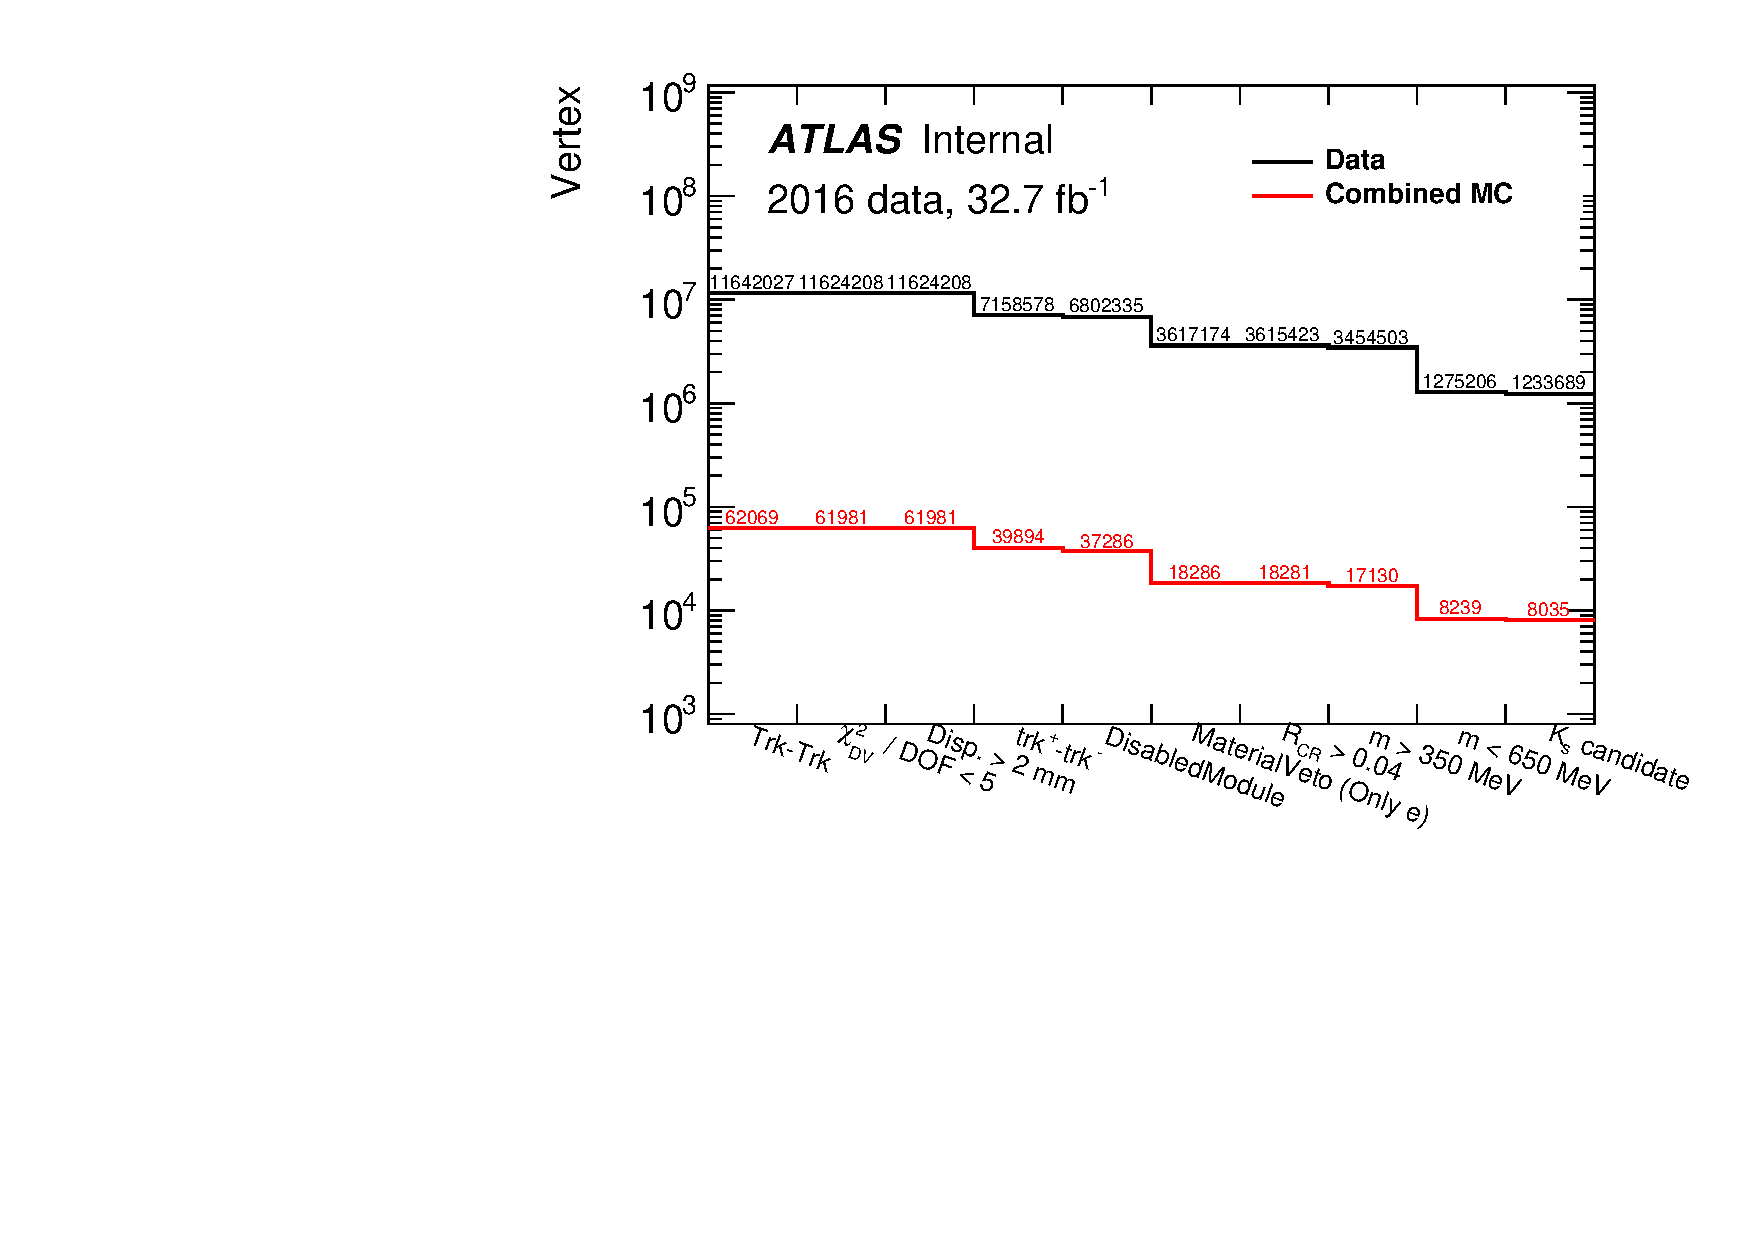
\includegraphics[width=0.60\textwidth]{figures/m_syst_Ks_cf.pdf}
	\centering
	\caption{Vertex cut flow applied on $K_{S}$ vertices in the data and MC samples}
	\label{fig:Ks_vertex_cutflow}
\end{figure}

After applying the event and $K_{S}$ vertex selection, the $K_{S}$ vertex distributions in the data are compared to the MC samples in Figure~\ref{fig:Ks_data_MC}. The data sample is normalized to the MC sample which has limited statistics. There are good agreements in the invariant mass, $p_{T}$, transverse, longitudinal position, and decay length of the vertices, except the pile-up distribution as expected.


\begin{figure}[!htb]
    \centering
    \subfloat[]{\label{subfig:Ks_m}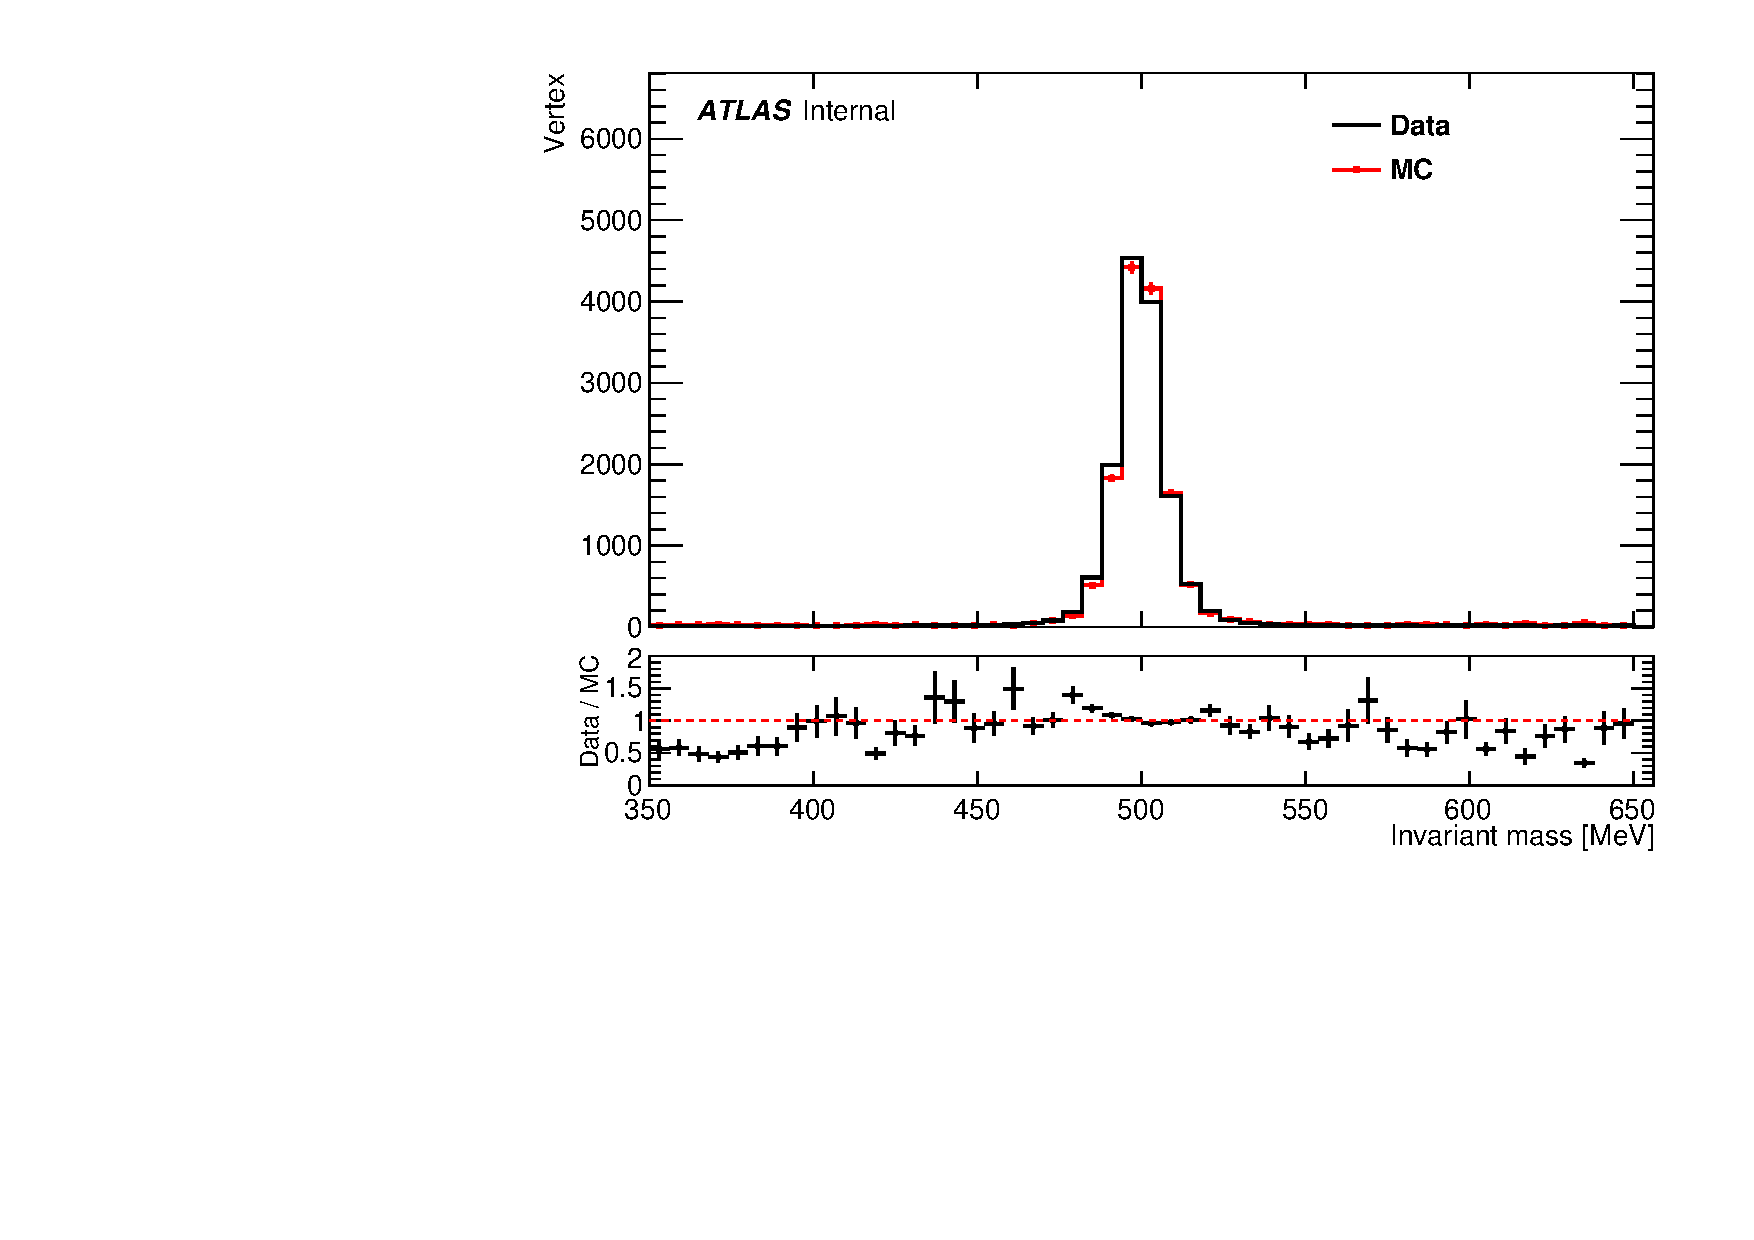
\includegraphics[width=0.45\textwidth]{figures/m_syst_Ks_M.pdf}}
    \subfloat[]{\label{subfig:Ks_pt}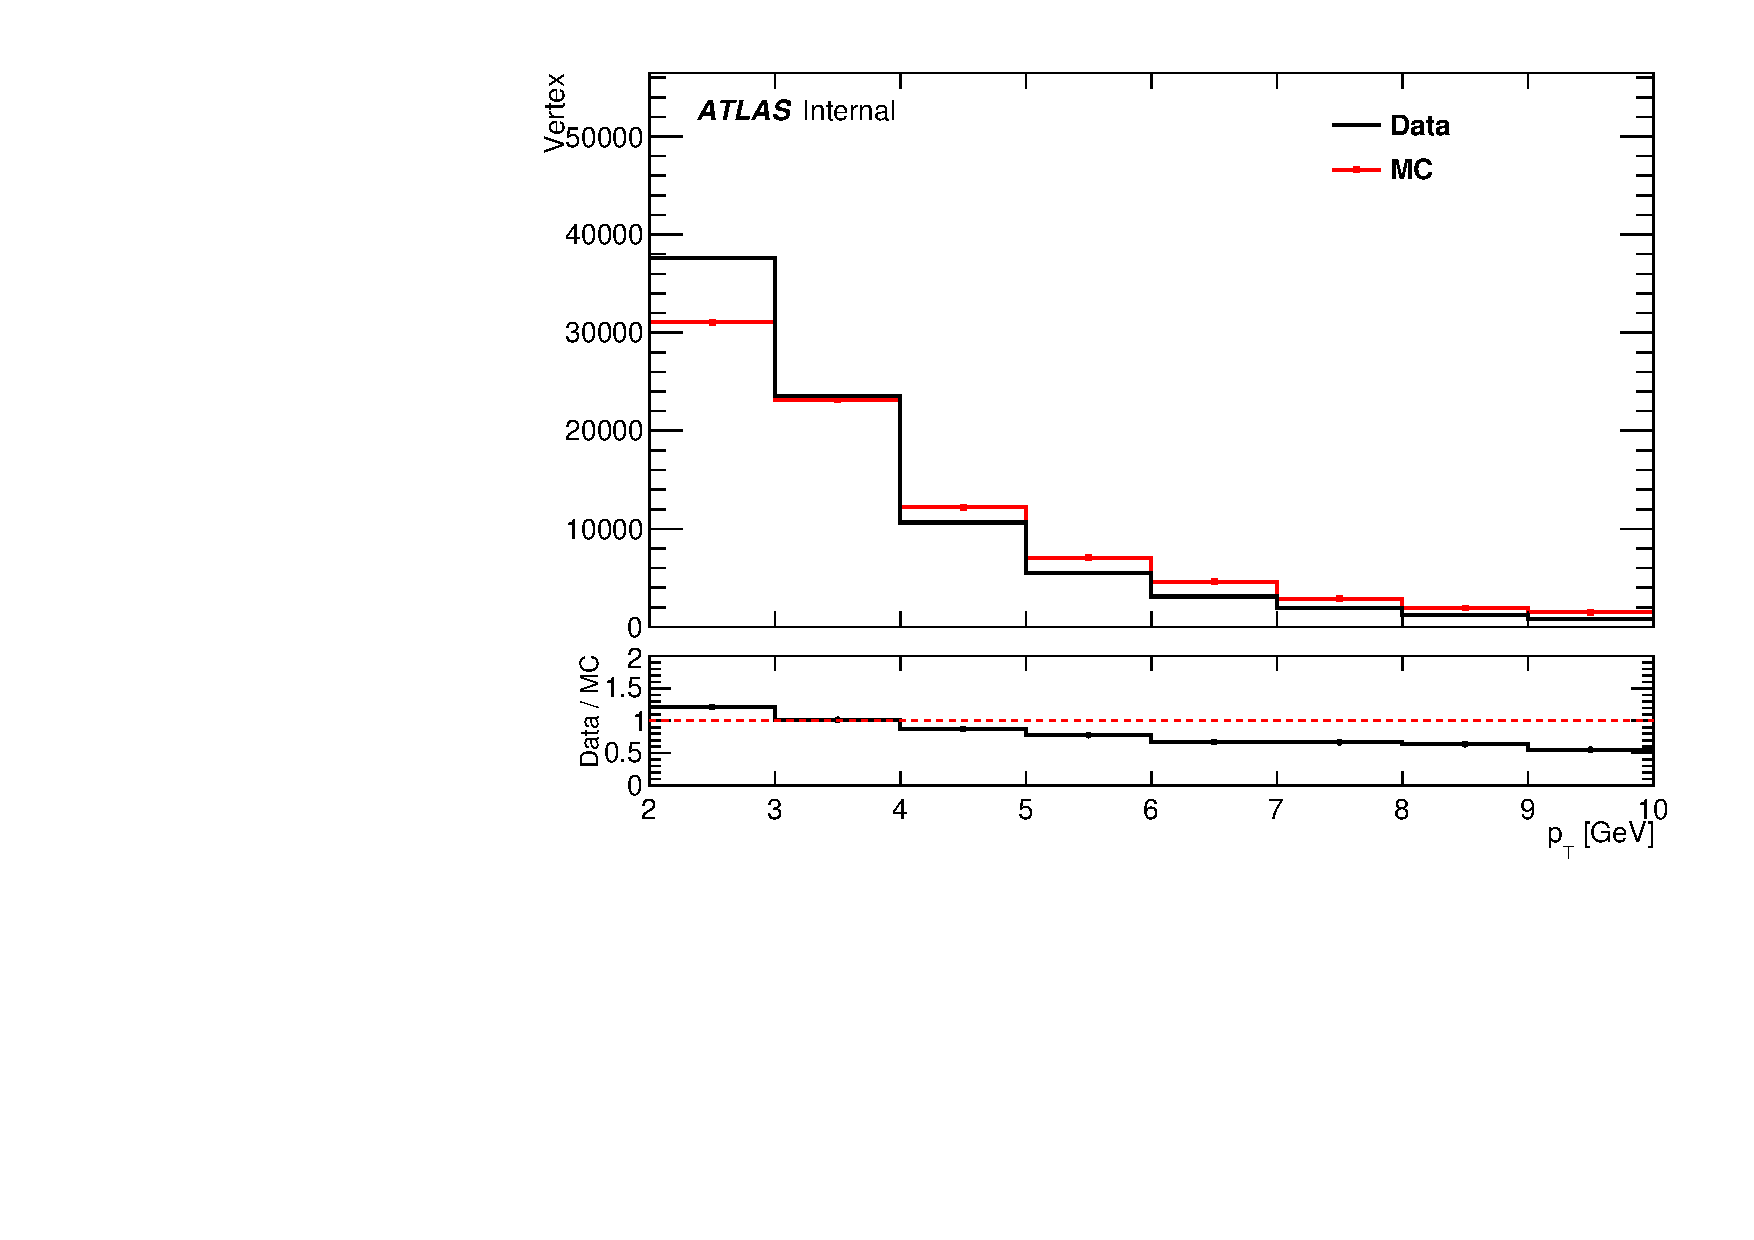
\includegraphics[width=0.45\textwidth]{figures/m_syst_Ks_pt.pdf}} \\
    \subfloat[]{\label{subfig:Ks_mu}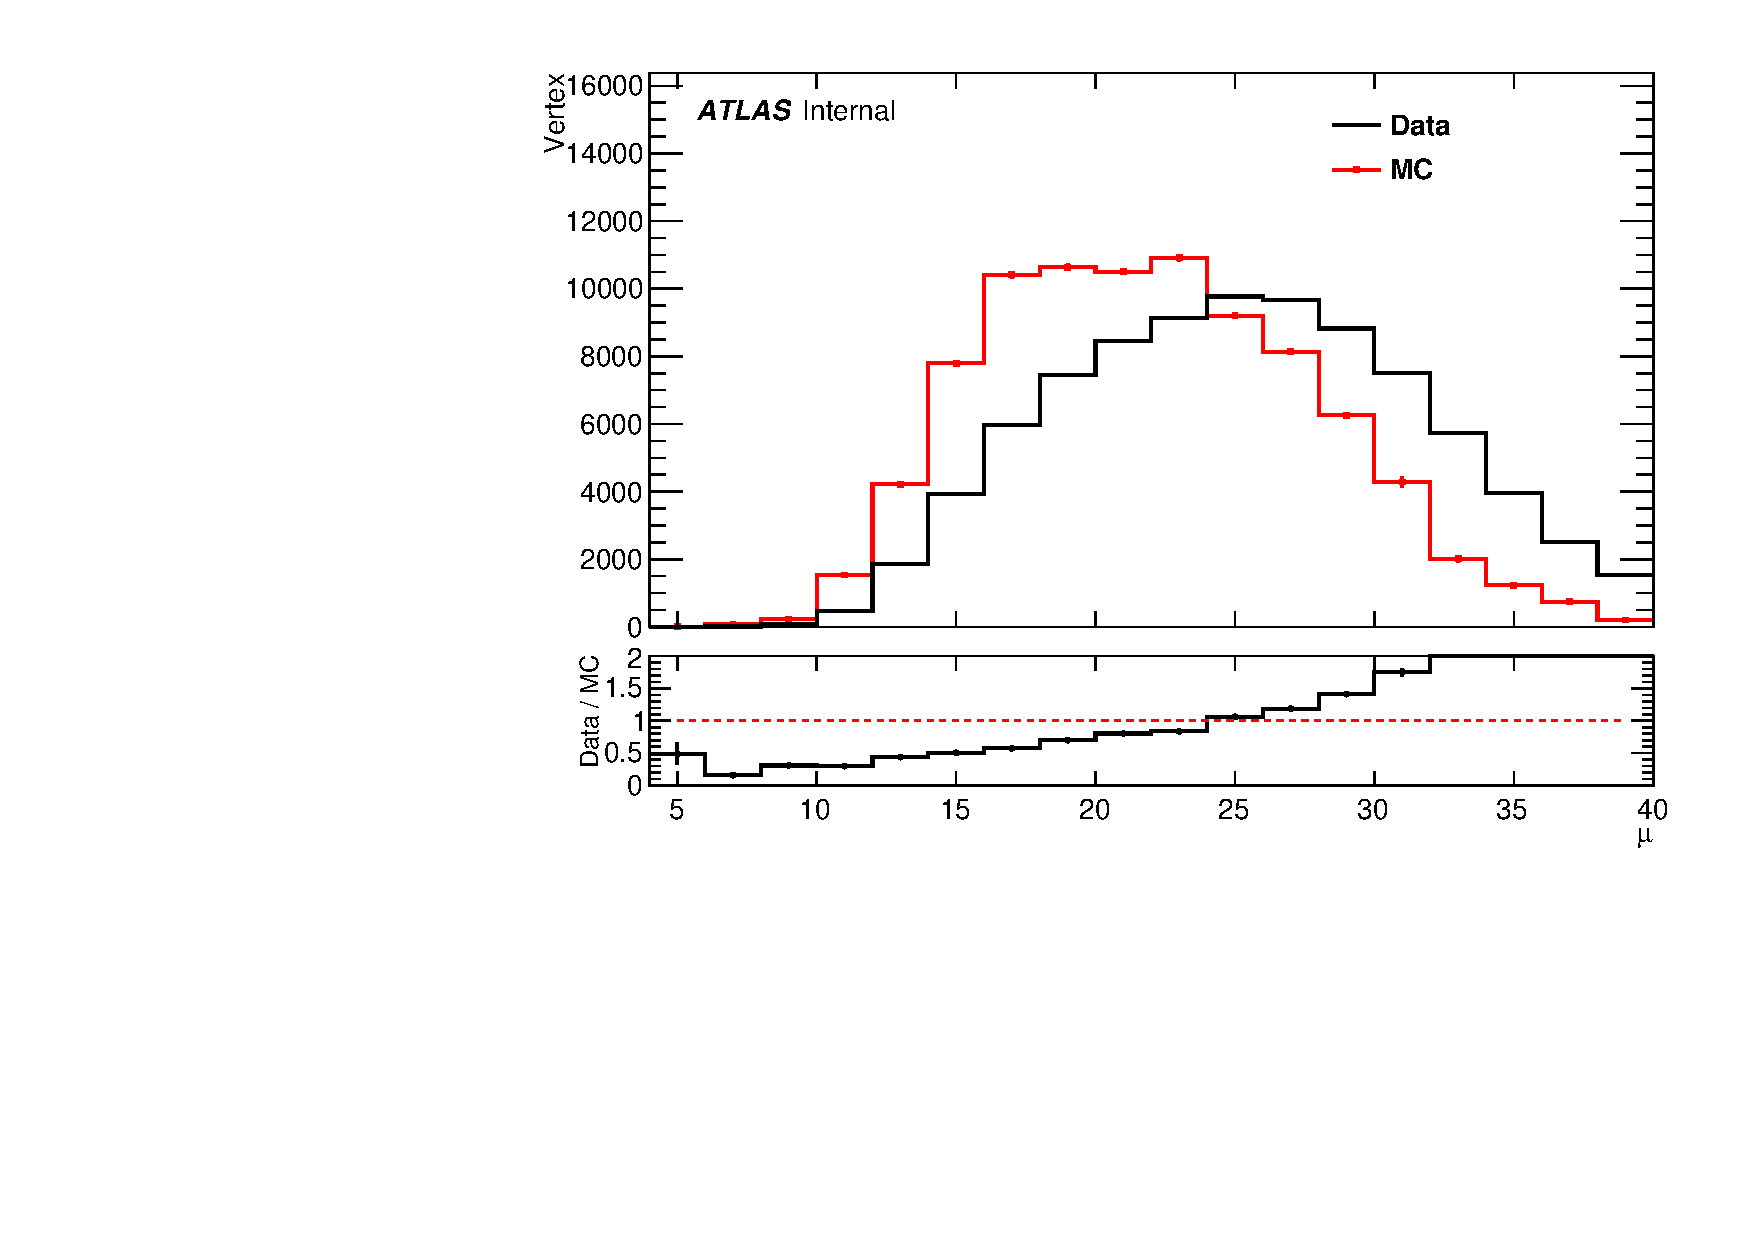
\includegraphics[width=0.45\textwidth]{figures/m_syst_Ks_mu.pdf}}
    \subfloat[]{\label{subfig:Ks_r}\includegraphics[width=0.45\textwidth]{figures/m_syst_Ks_r.pdf}}  \\
    \subfloat[]{\label{subfig:Ks_z}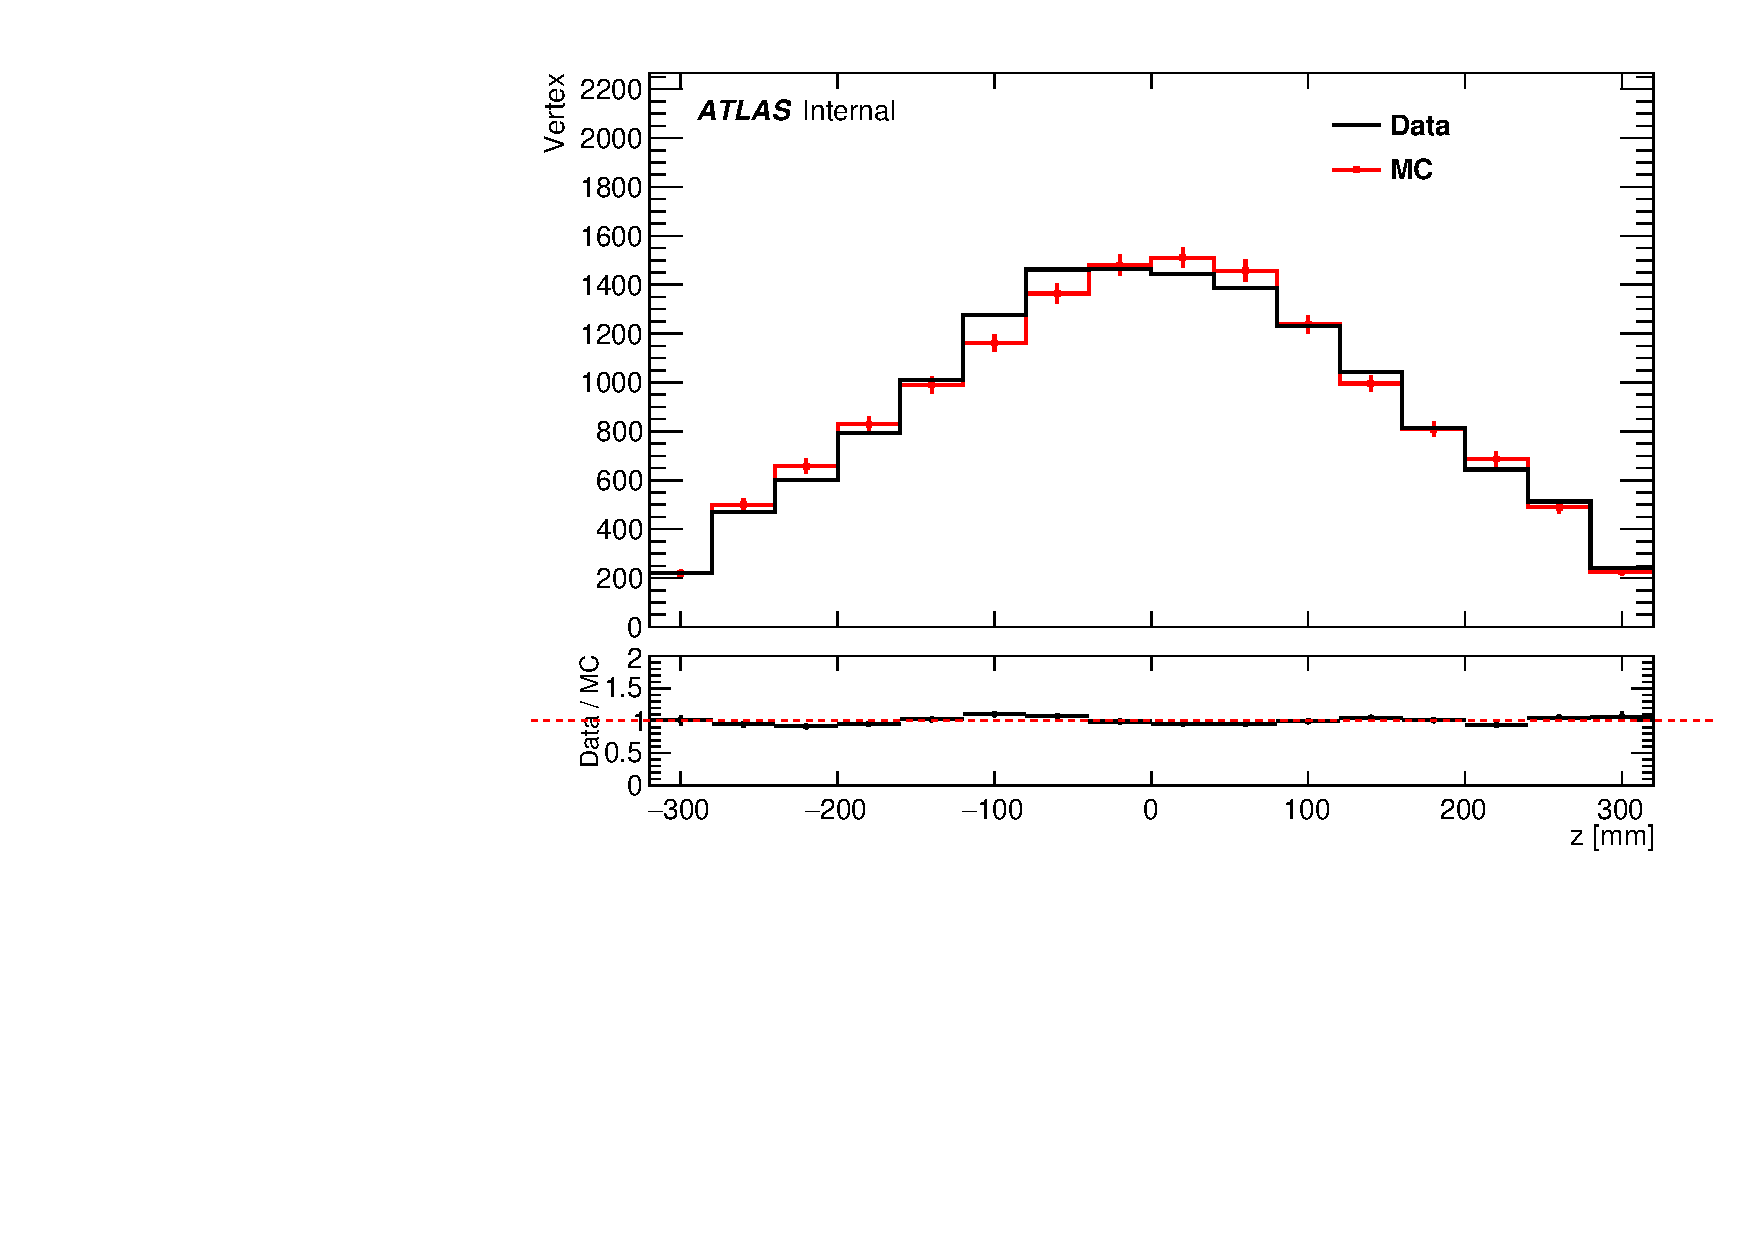
\includegraphics[width=0.45\textwidth]{figures/m_syst_Ks_z.pdf}} 
    \subfloat[]{\label{subfig:Ks_l}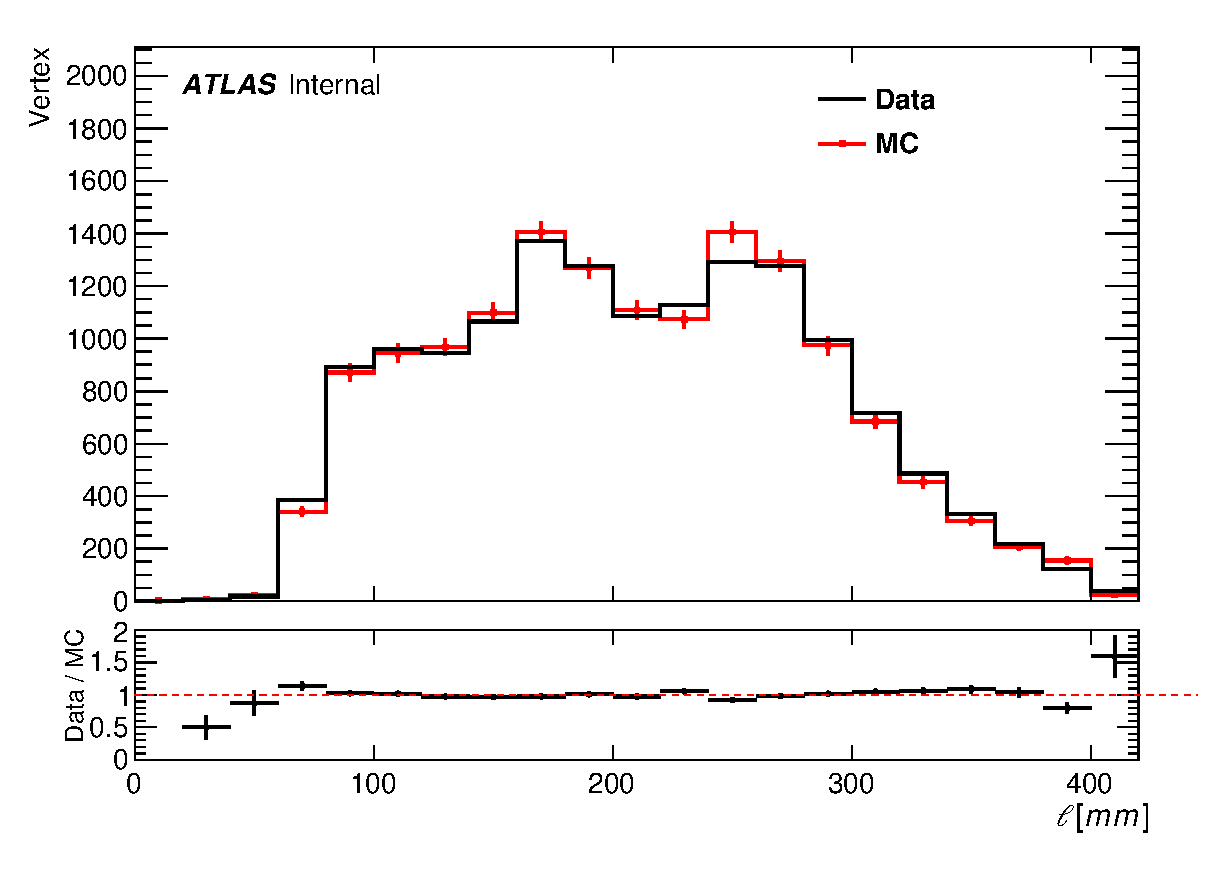
\includegraphics[width=0.45\textwidth]{figures/m_syst_Ks_l.eps}} \\
    \caption{Comparison of the (a) invariant mass, (b) $p_{T}$, (c) $\mu$, (d) transverse, (e) longitudinal position, and (f) decay length of $K_{S}$ in the data with the MC samples. Data is normalized to MC. In (d), the red dashed lines indicate the four Pixel layers and the first layer of SCT. The green dotted lines indicate the Inner Support Tube (45.5 mm) and Pixel Support Tube (229 mm).}
    \label{fig:Ks_data_MC}
\end{figure}

$K_{S}$ vertices found in the data and MC samples are binned in decay radius, $r$, and the $K_{S}$ yields in each bin are estimated from a fit using Breit-wigner. Figure~\ref{fig:Ks_fit} shows a few representative $K_{S}$ mass distributions (others are included in Appendix~\ref{app:syst_Ks_fit}). Background is negligible and hence not included in the fit. The estimated $K_{S}$ yields are normalized to the number of $K_{S}$ found in the lowest $r$ bin since the expected number of $K_{S}$ in the data samples is unknown. 

%\begin{figure}[tb]
\begin{figure}[!htb]
    \centering
    \subfloat[]{\label{subfig:Ks_fit_MC_1}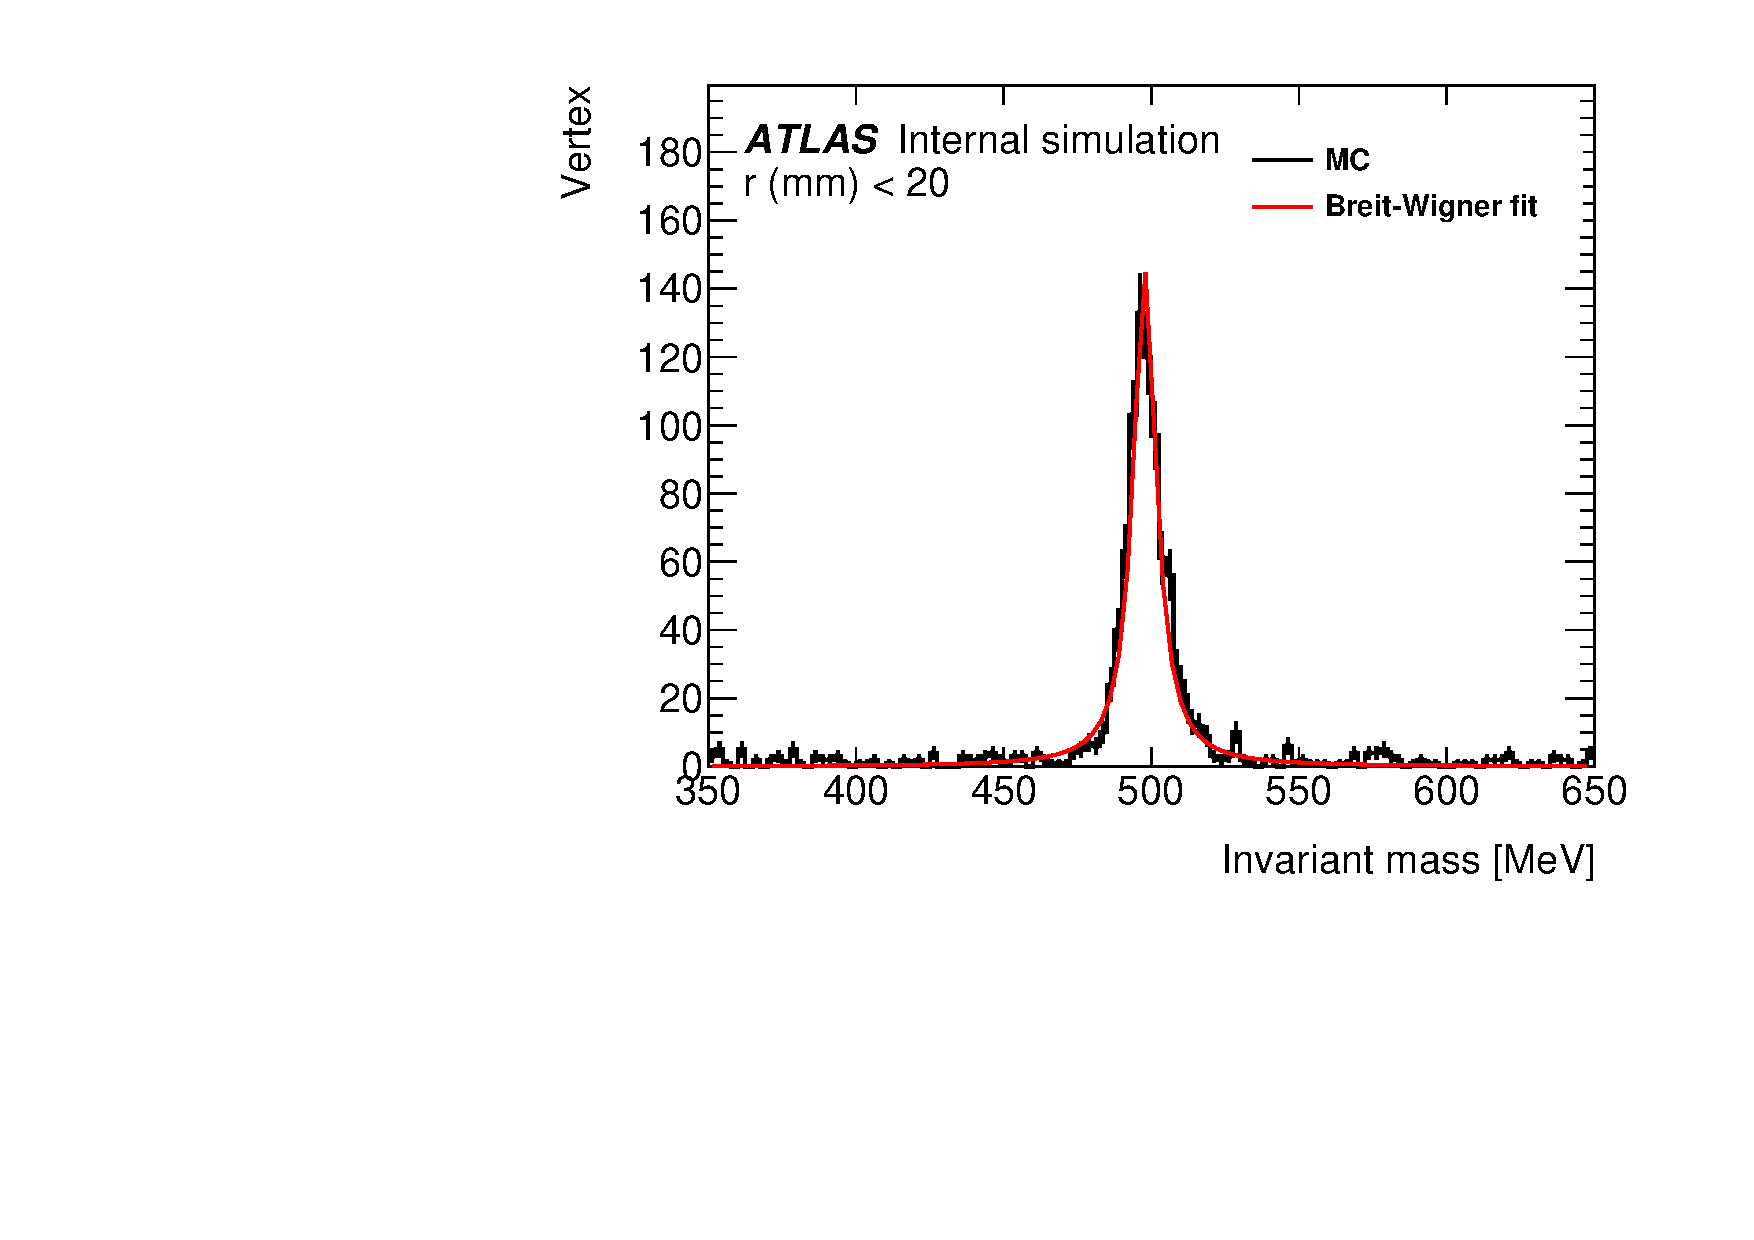
\includegraphics[width=0.45\textwidth]{figures/m_syst_Ks_Combined_MC_1}}
    \subfloat[]{\label{subfig:Ks_fit_MC_2}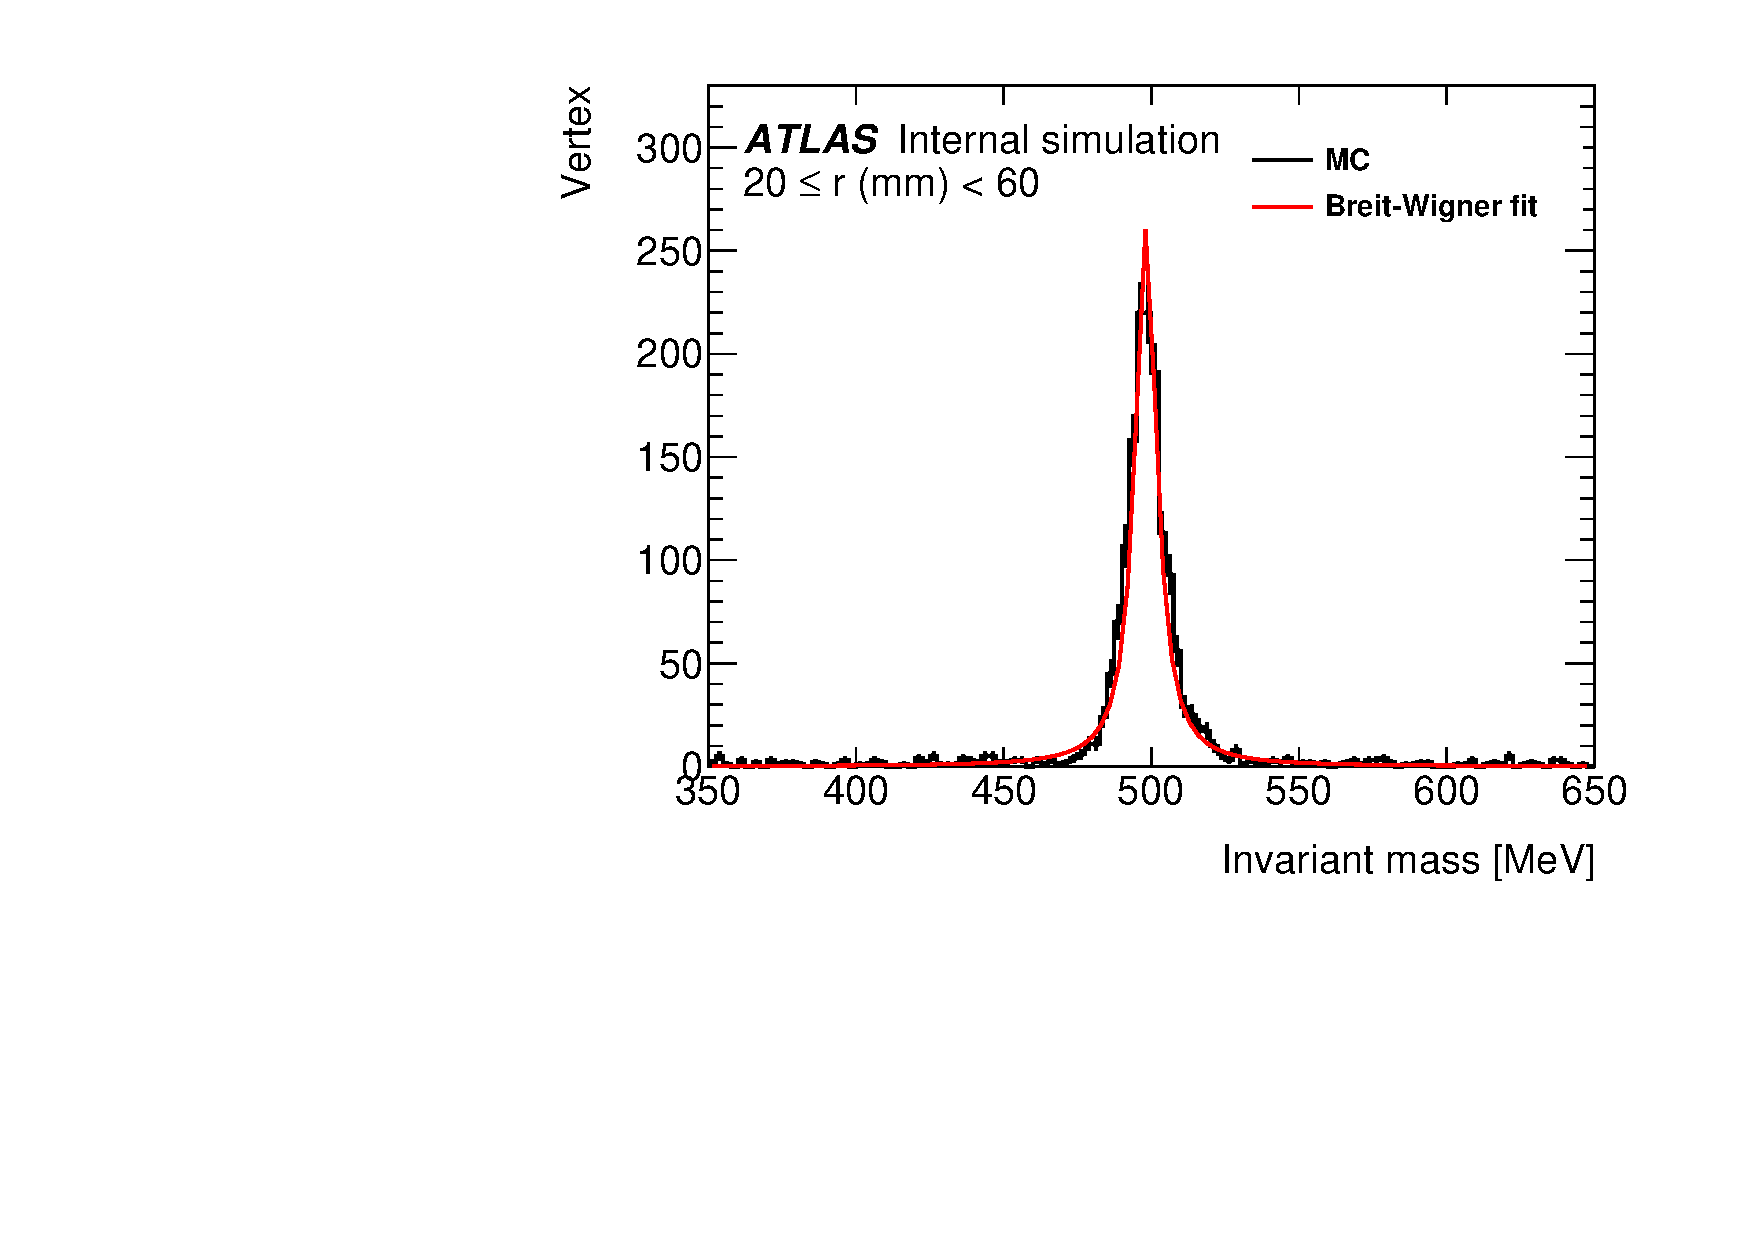
\includegraphics[width=0.45\textwidth]{figures/m_syst_Ks_Combined_MC_2}} \\
    \subfloat[]{\label{subfig:Ks_fit_Data_1}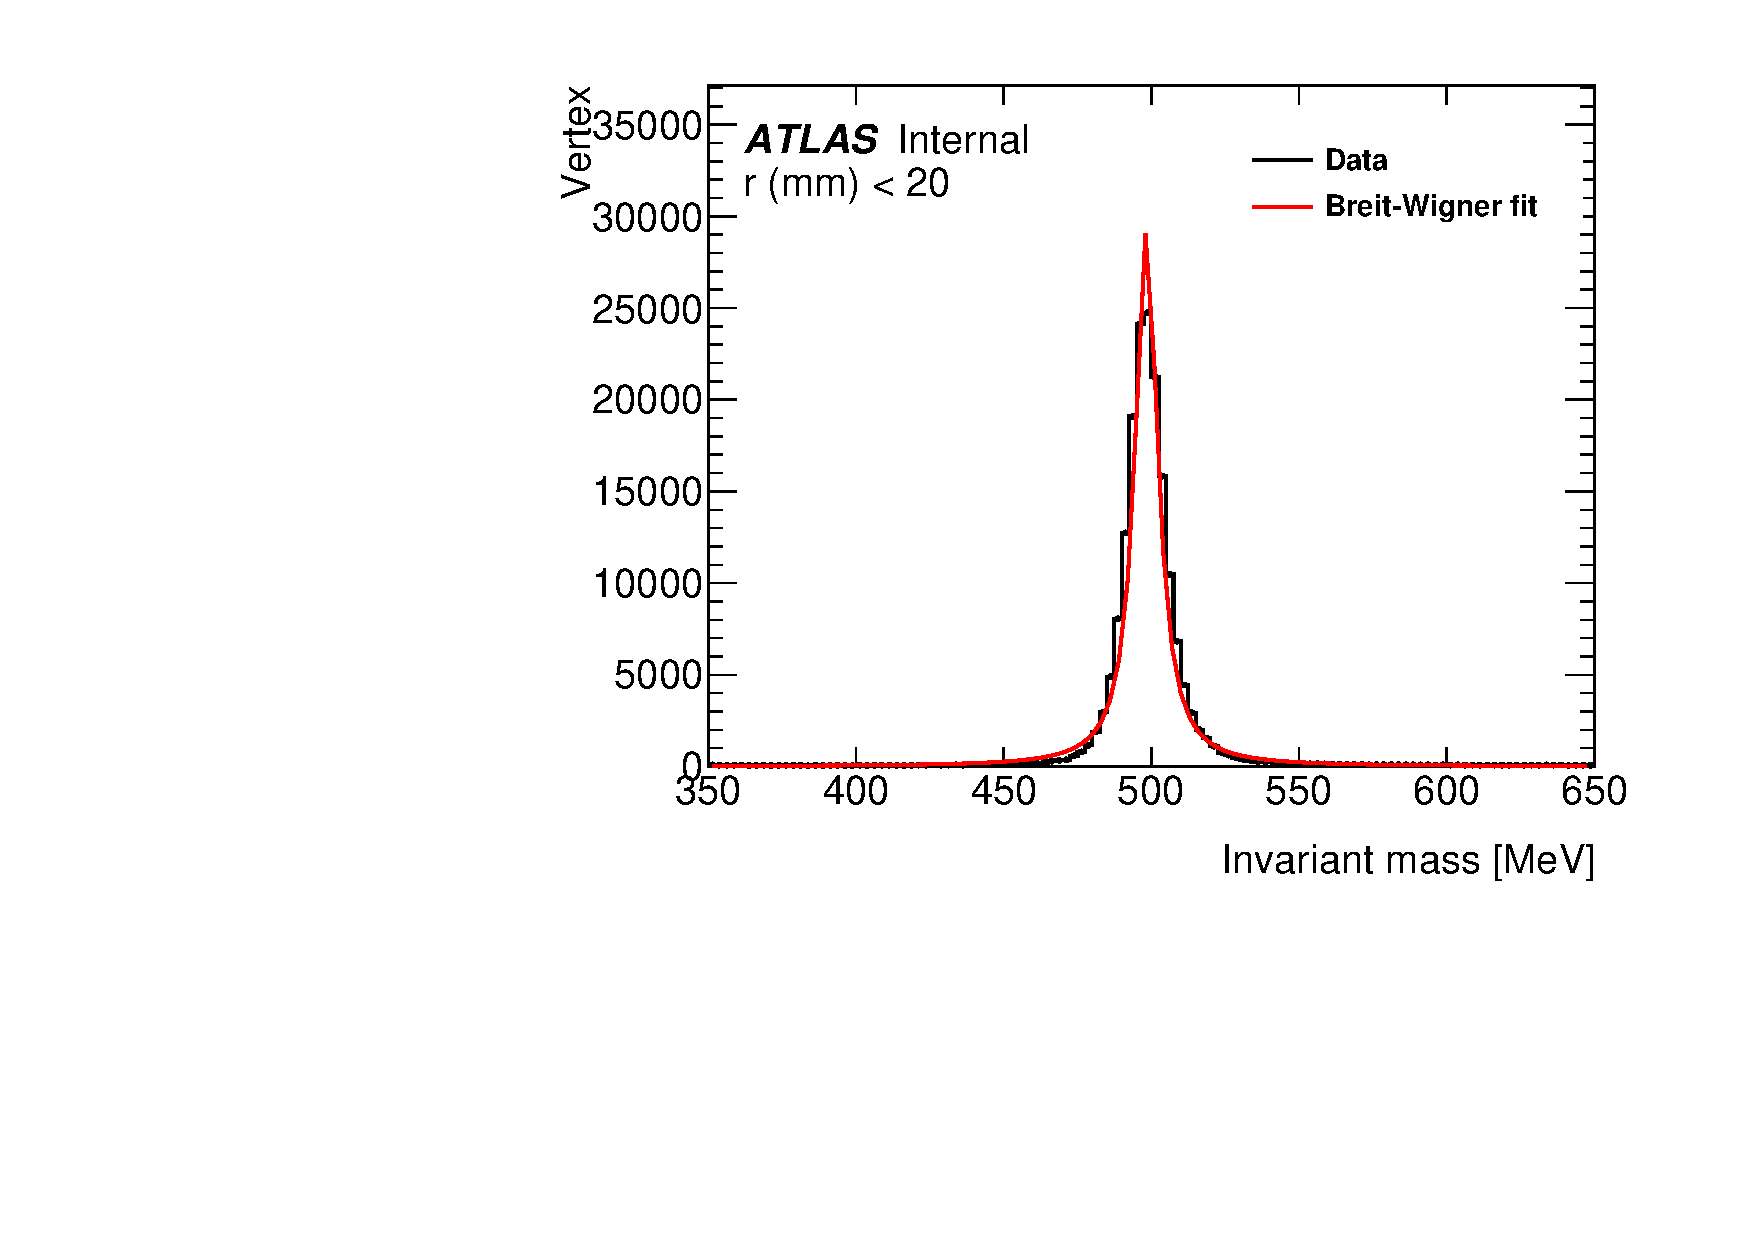
\includegraphics[width=0.45\textwidth]{figures/m_syst_Ks_Data_1}}
    \subfloat[]{\label{subfig:Ks_fit_Data_2}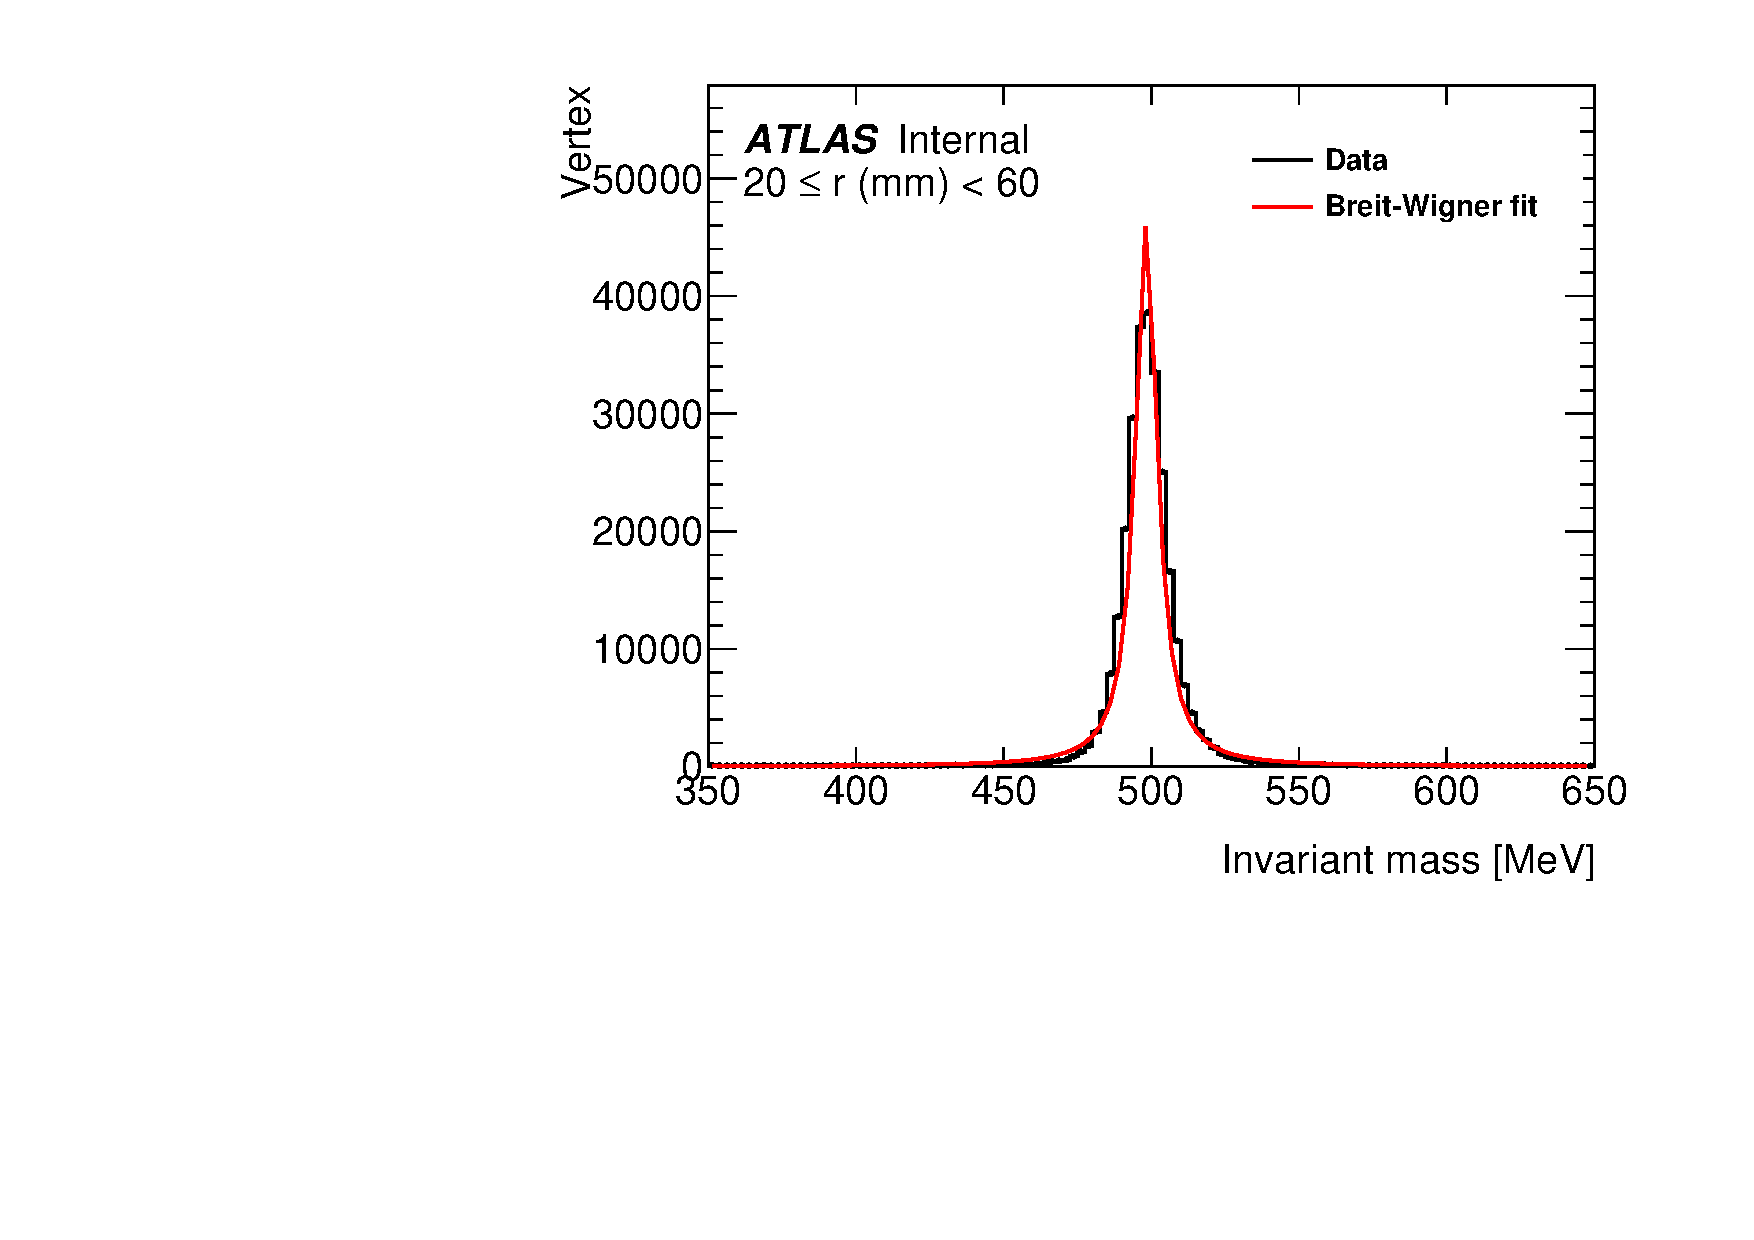
\includegraphics[width=0.45\textwidth]{figures/m_syst_Ks_Data_2}}
    \caption{Representative distributions of the $K_{S}$ invariant mass for (a) $r$ < 20 mm, and (b) 20 $<r<$ 60 mm in the background MC sample. The corresponding plots from the data sample are shown in (c) and (d). The mass distributions are fitted with a Breit-Wigner.}
    \label{fig:Ks_fit}
\end{figure}

%The systematic uncertainty in the lowest bin is taken from the run 2 study \cite{Aad:2011hd}. 
%The ratio of $K_{S}$ vertex yields in each bin of $r$ to $K_{S}$ vertex yields in the lowest $r$ bin is compared between the data and the background MC samples in Figure~\ref{fig:Ks_double_ratio}.
The $K_{S}$ yield, normalized to the yield with $r <$ 20 mm, is compared to the MC in Figure~\ref{fig:Ks_double_ratio}. The lower pane shows the double ratio,

\begin{equation}
\frac{N^{\mathrm{data}}_{R}}{N^{\mathrm{data}}_{R_{0}}} \bigg/ \frac{N^{\mathrm{MC}}_{R}}{N^{\mathrm{MC}}_{R_{0}}}
\label{eq:ks_double_ratio}
\end{equation}

which shows deviation from unity with increase of $r$. The difference in yield is then convoluted with the $r$ distribution of $Z'$ to estimate the systematic uncertainty in tracking and vertexing.

\begin{figure}[!htb]
	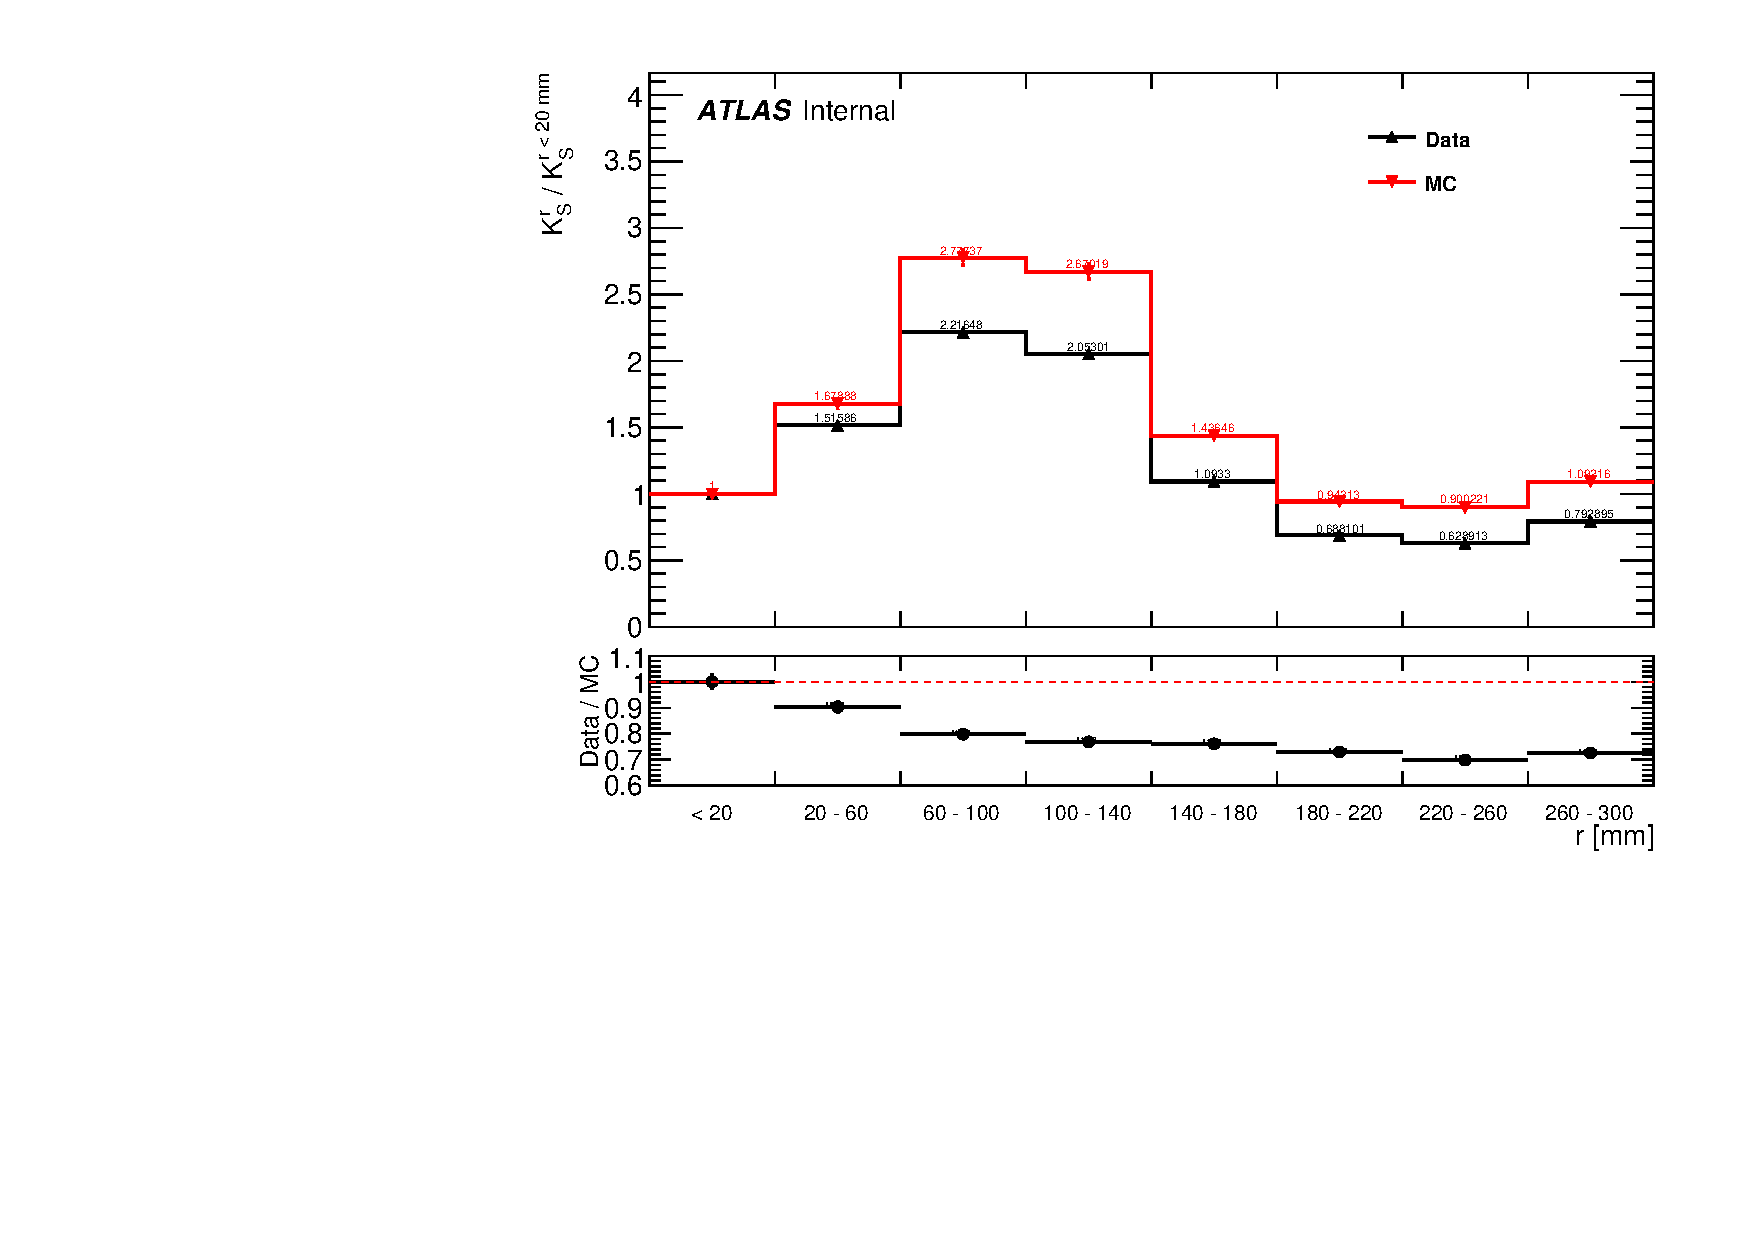
\includegraphics[width=0.50\textwidth]{figures/m_syst_Ks_ratio.pdf}
	\centering
	\caption{The radial distribution of $K_{S}$ yield, normalized to the lowest $r$ bin in the data and MC samples. The lower pane shows the double ratio as defined in the text.}
	\label{fig:Ks_double_ratio}
\end{figure}



\newpage

\begin{align}
    %S_{xx\rightarrow \mu x} &= N_{\mu x}^{obs} / N_{\mu x}^{est}, \nonumber \\
    %S_{xx\rightarrow \ex}   &= N_{e x}^{obs} / N_{e x}^{est}
    S_{xx\rightarrow \mu x} &= \frac{N_{\mu x}^{obs}}{N_{\mu x}^{est}}, \nonumber \\
    S_{xx\rightarrow \ex}   &= \frac{N_{e x}^{obs}}{ N_{e x}^{est}}
\label{eq:random_crossing_scale_factor}
\end{align}

















\newpage

\section{Systematic uncertainties in trigger efficiency}
\label{sec:syst:trigger}

Systematic uncertainties in lepton triggers are usually measured with tag-and-probe studies on $Z$+jet where most leptons have small impact parameters. However, because the leptons originating from displaced vertices tend to have large impact parameters, the standard systematics on triggers provided by the performance groups cannot be applied. In the following, the systematic uncertainties in the lepton triggers are estimated using tag-and-probe method on the data and $Z$+jets MC samples. 

The estimated systematic uncertainties are valid only if the trigger efficiencies do not depend on impact parameters or if this dependence is modelled reasonable well in simulations. Therefore, the efficiencies of the single photon and single muon triggers listed on Table~\ref{table:triggers} are estimated using the signal MC samples and shown in Figure~\ref{fig:signal_TrigEff}.

The photon trigger efficiency is consistent for both the transverse and the longitudinal impact parameter. The muon trigger efficiency starts to decrease for large impact parameters, $|\dzero| \approx 120~\si{\mm}$ and $|\zzero| \approx 200~\si{\mm}$. However, the decreasing muon efficiency at very large impact parameters is neglected since the fraction of reconstructed muons with such large impact parameters is less than 10\% at the lifetime of $c\tau=100~\si{\mm}$.


\begin{figure}[!htp]
    \centering
    \subfloat[]{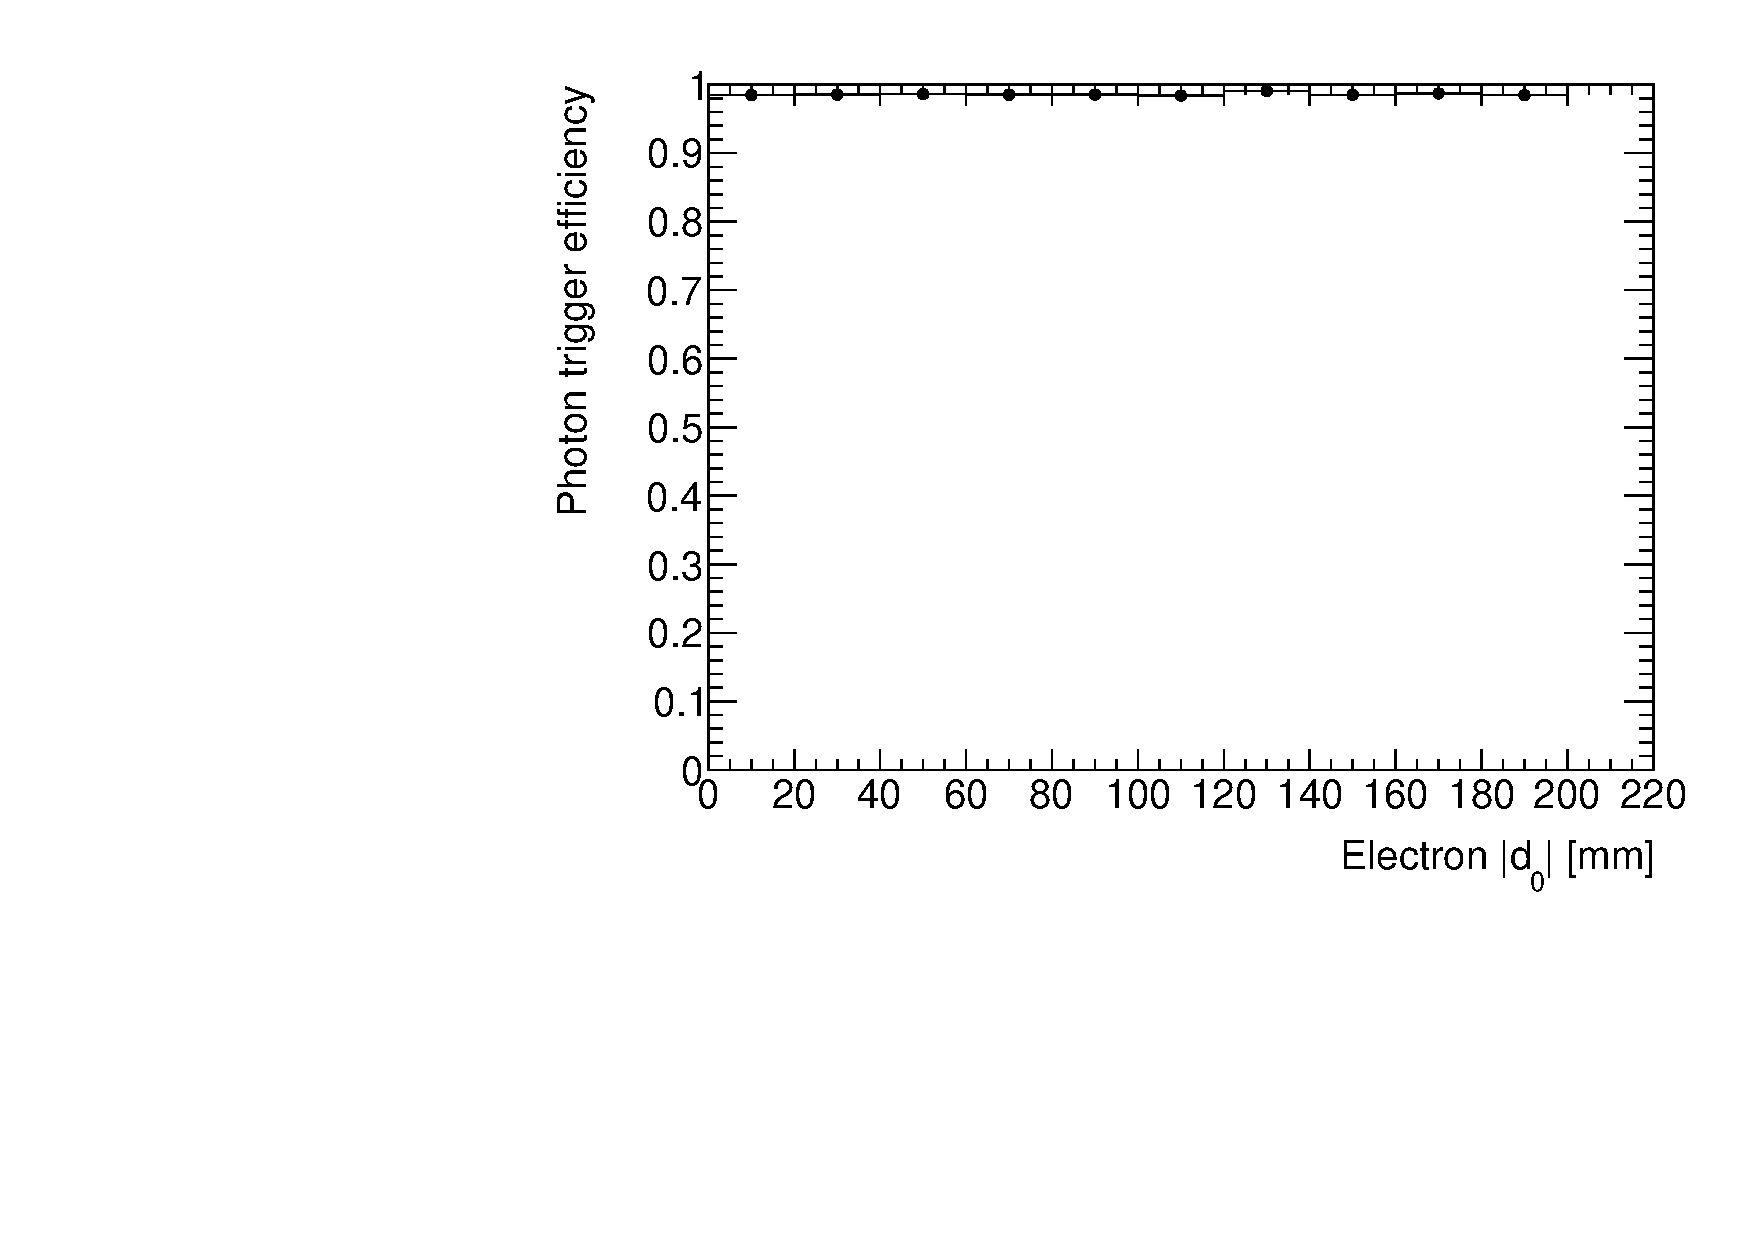
\includegraphics[width = 0.44 \textwidth]{figures/TrigEff/signal/eff_siph_d0.pdf}}
    \subfloat[]{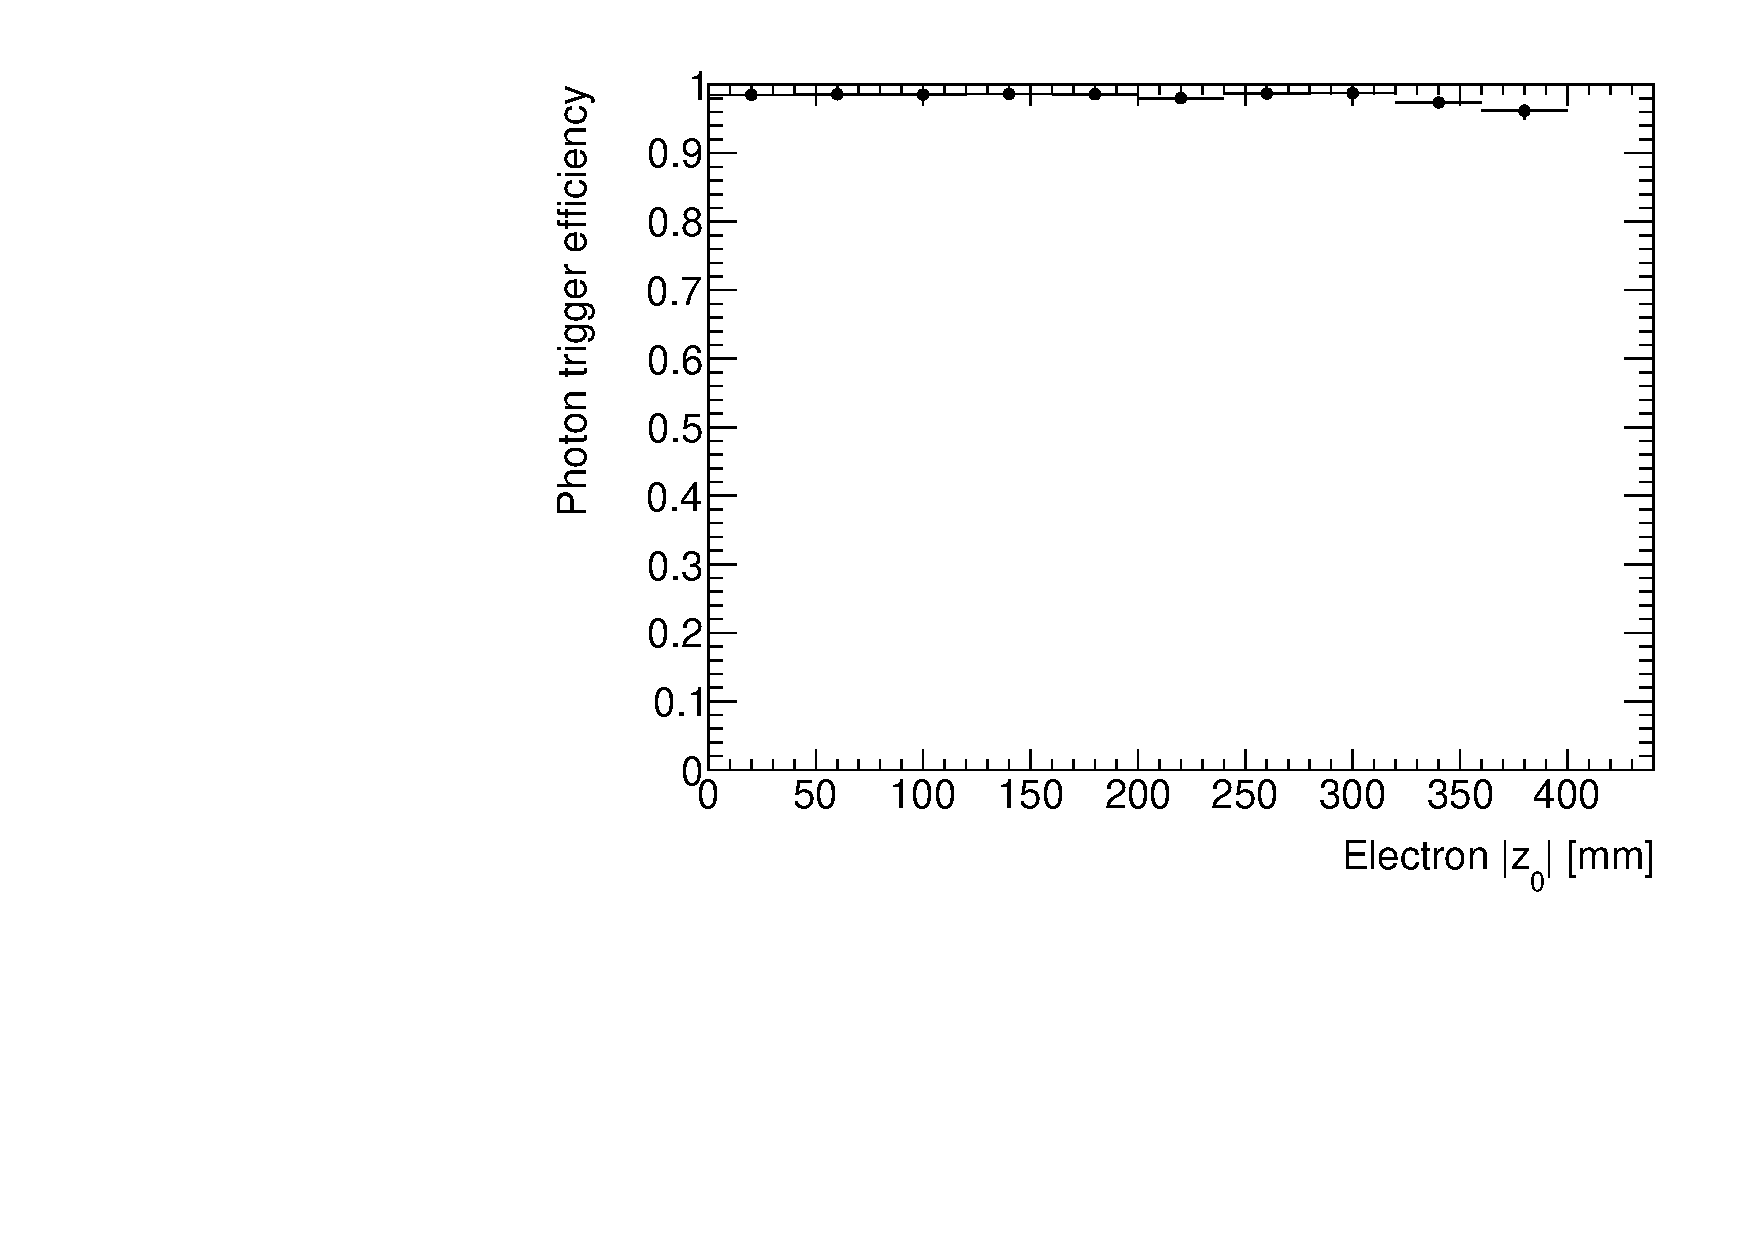
\includegraphics[width = 0.44 \textwidth]{figures/TrigEff/signal/eff_siph_z0.pdf}} \\
    \subfloat[]{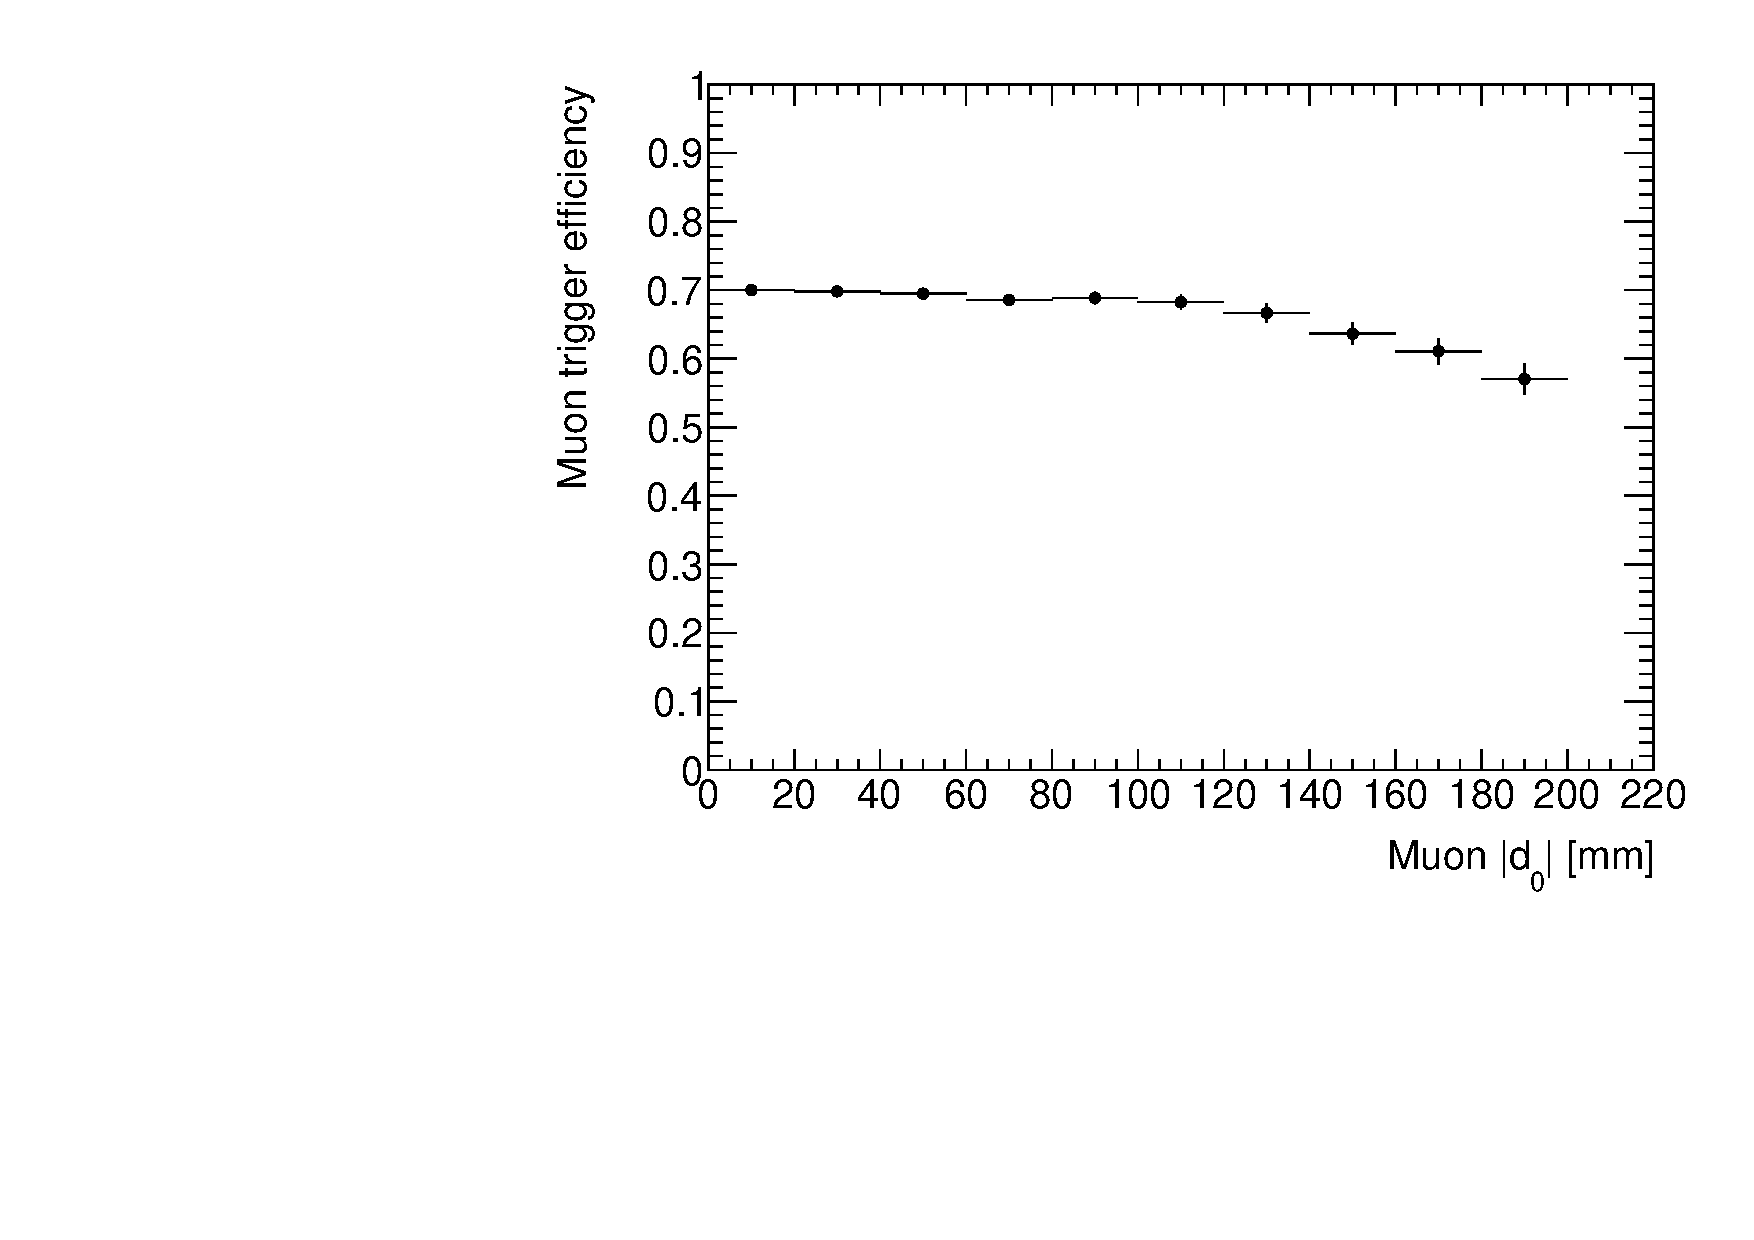
\includegraphics[width = 0.44 \textwidth]{figures/TrigEff/signal/eff_simu_d0.pdf}}
    \subfloat[]{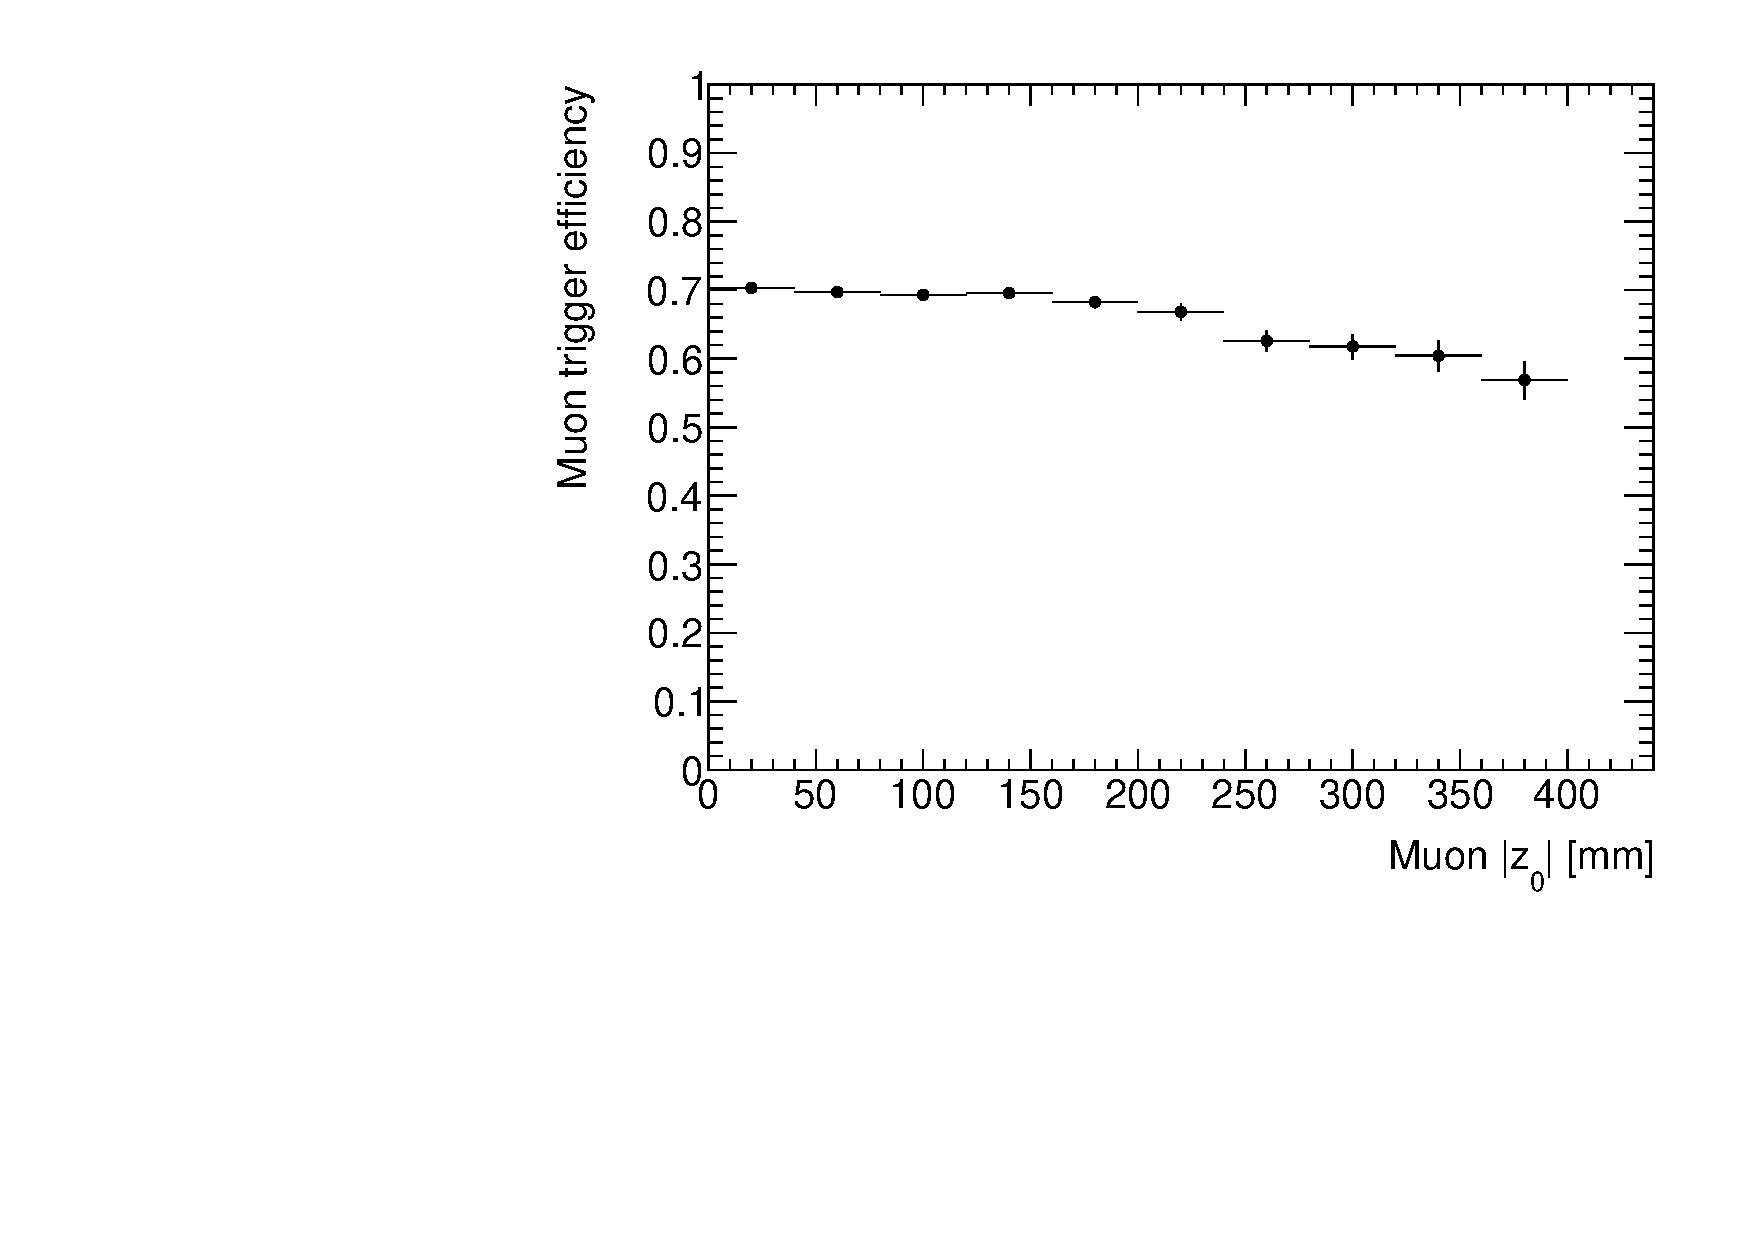
\includegraphics[width = 0.44 \textwidth]{figures/TrigEff/signal/eff_simu_z0.pdf}}
    \caption{The efficiency of the single photon trigger in electron (a) $|\dzero|$ and (b) $|\zzero|$. The corresponding plots of the single muon trigger are shown in (c) and (d).}
    \label{fig:signal_TrigEff}
\end{figure}



\subsection{Photon triggers}
\label{subsect:photonTrigEff}

The systematic uncertainties of the single photon and the di-photon triggers are estimated with a standard tag and probe method on $Z\rightarrow ee$ events both in data and MC samples. The di-photon trigger (\texttt{HLT\_2g50\_loose}) is studied using the single muon trigger (\texttt{HLT\_g50\_loose}) with the same $p_{T}$ threshold. The selection criteria of electron tag-and-probe candidates are listed in Table~\ref{tab:ZeeSelection}. In addition, pairs are required to have opposite signs and to satisfy the mass requirement ($|m_{e^{+}e^{-}} - m_{Z}| < 10~\si{\GeV}$) and the isolation requirement of $\DeltaR(\mathrm{tag}, \mathrm{probe}) > 0.4$. 

\begin{table}[!htb]
	\centering
	\begin{tabular}{ccc}
		\hline
		\hline
		Selection & Tag & Probe \\
		\hline
		$p_{T}$ (GeV) $>$ & 27 & 30 \\
		Trigger matched & \texttt{HLT\_e26\_lhtight\_nod0\_ivarloose} & --- \\
		$|\eta|$ & $<$ 1.37 or ($>$ 1.52 and $<$ 2.47) & < 2.47 \\
		Identification & TightLH & LooseLHNoD0 \\
		Object quality & yes & yes \\
		Track isolation & yes & --- \\
		Jet veto & --- & yes \\
		\hline
		\hline
	\end{tabular}
	\caption{Selection criteria for tag-and-probe electrons in $Z$+jets studies.}
	\label{tab:ZeeSelection}
\end{table}

The invariant mass distributions of the tag-and-probe pairs found in the data and MC samples are shown in Figure~\ref{fig:PhotonTrigMass}. The shape of distribution is in good agreement with negligible background for both triggers. Therefore, no background subtraction is performed in the calculation of the trigger efficiencies, 

\begin{equation}
	\label{eq:TrigEff}
    \epsilon_{\mathrm{trigger}} = \frac{\textrm{Number of probes matched to trigger}}{\textrm{Number of all probes}}.
\end{equation}

\begin{figure}[!htb]
    \centering
    \subfloat[]{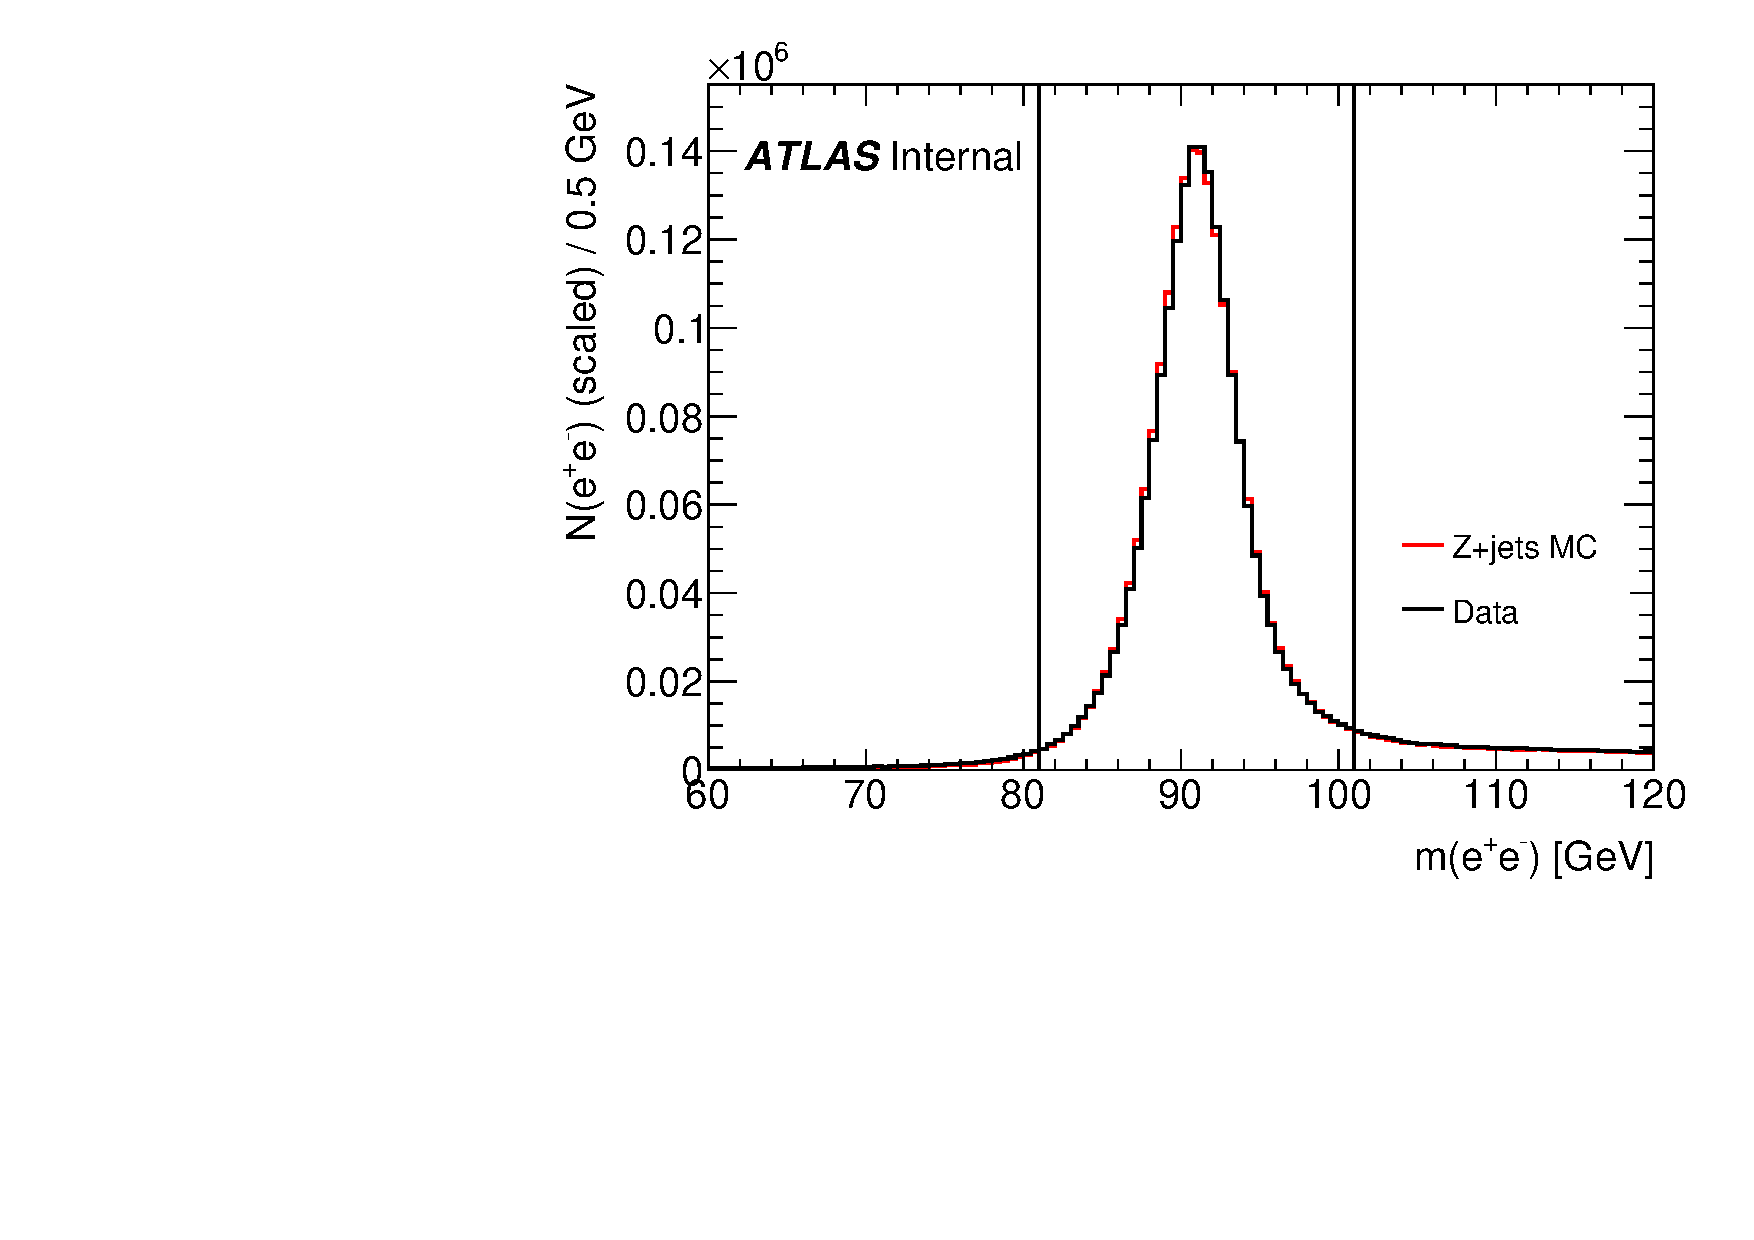
\includegraphics[width = 0.44 \textwidth]{figures/PhotonTrigEff/diph_mass.pdf}}
    \subfloat[]{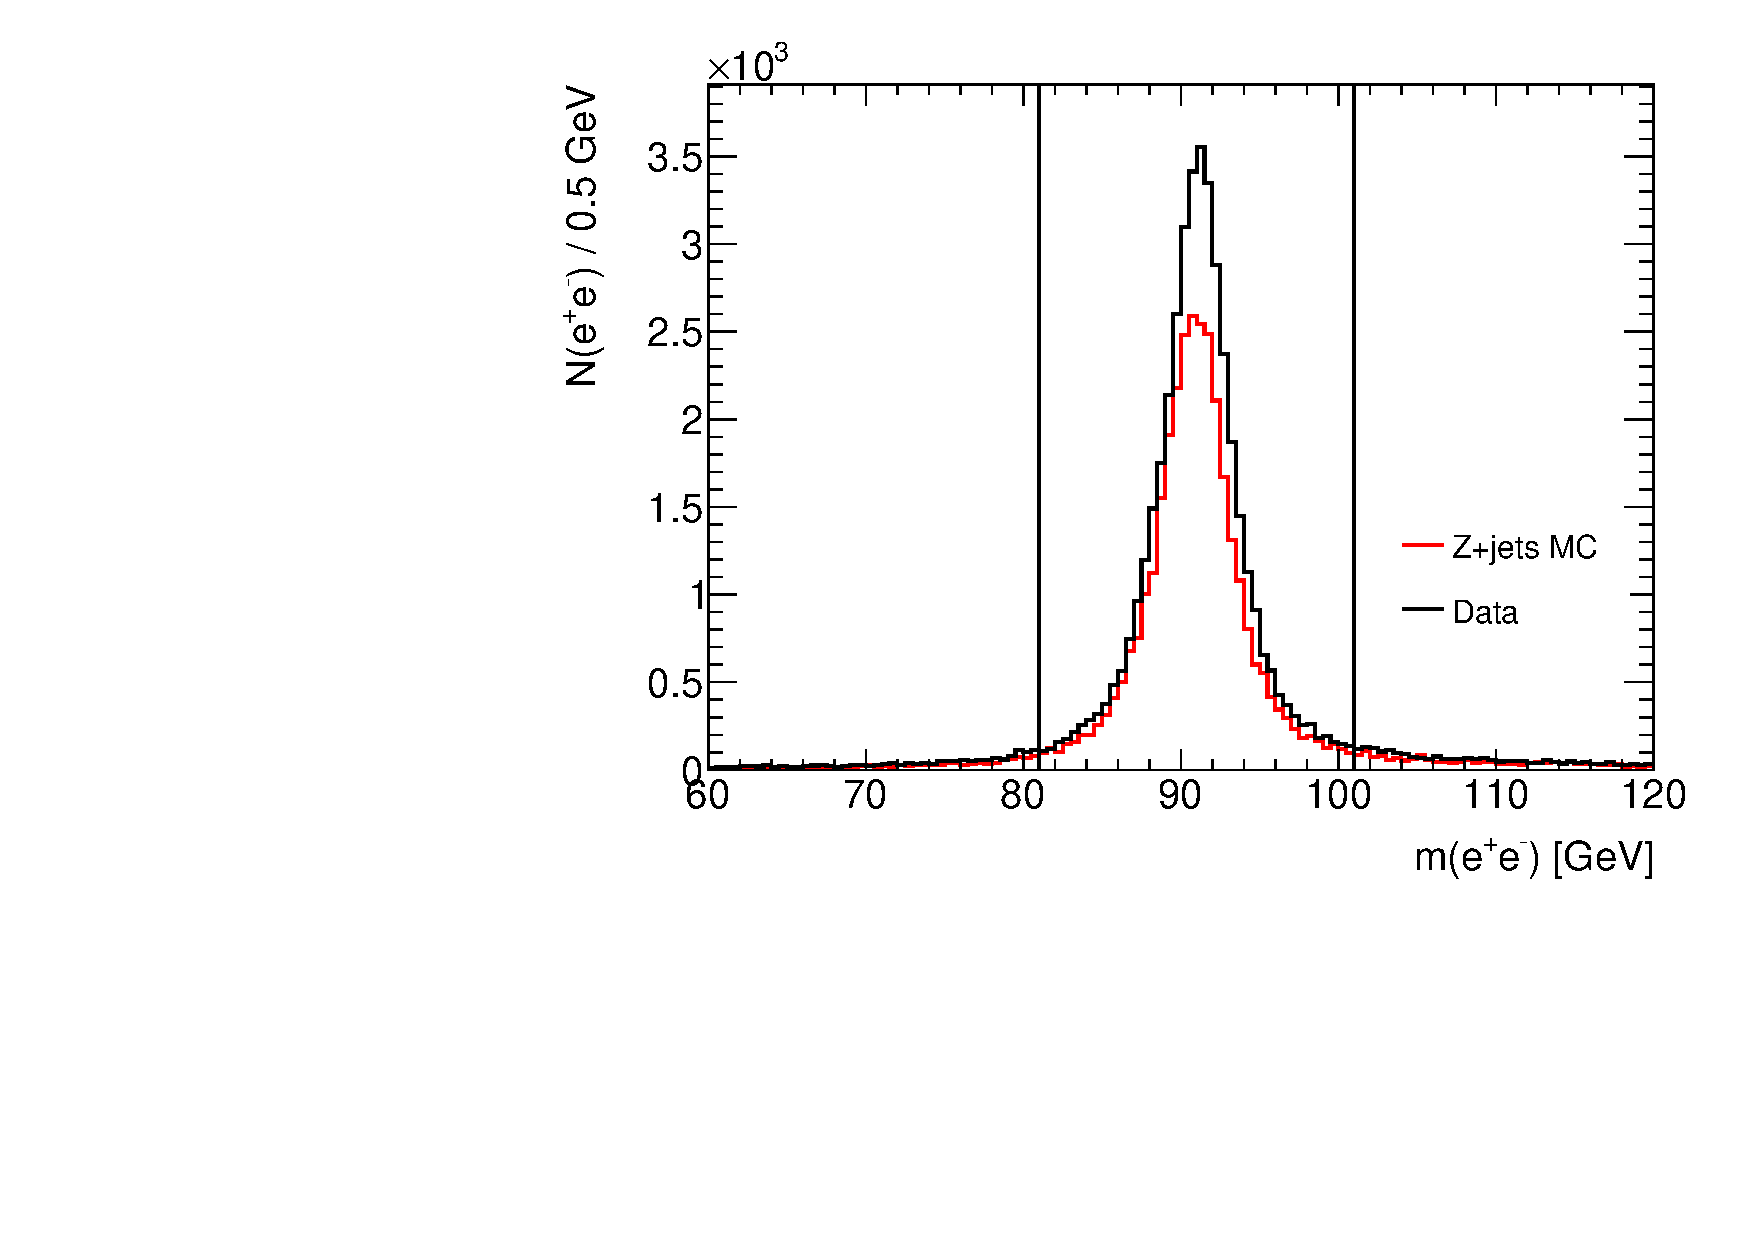
\includegraphics[width = 0.44 \textwidth]{figures/PhotonTrigEff/siph_mass.pdf}}
    \caption{Invariant mass distributions of the tag-and-probe electron pairs used to study the efficiencies of the (a) \texttt{HLT\_g50\_loose} and (b) \texttt{HLT\_g140\_loose} trigger in the data and $Z$+jets MC samples. Only the pairs with a probe electron in the plateau region of Figure~\ref{fig:PhotonTrigEff:di_pt} and~\ref{fig:PhotonTrigEff:si_pt} are considered.
    }
    \label{fig:PhotonTrigMass}
\end{figure}

The selected tag-and-probe electrons are used to estimate the efficiencies of photon triggers, shown as a function of probe $p_{T}$, $\eta$, and $|\zzero|$ in Figure~\ref{fig:PhotonTrigEff}. The efficiencies in $p_{T}$ show that the \texttt{HLT\_g50\_loose} plateau starts at $55 \si{\GeV}$, and \texttt{HLT\_g140\_loose} plateau starts at $148 \si{\GeV}$. The efficiencies in $\eta$ show good agreement between data and MC for electrons reconstructed inside the barrel, whereas small discrepancy in efficiencies are shown for electrons at the boundary regions and in the end-cap regions. Also, the efficiency in $|\zzero|$ shows no dependence of the photon trigger efficiencies on $|\zzero|$

\begin{figure}[!htb]
    \centering
    \subfloat[]{\label{fig:PhotonTrigEff:di_pt}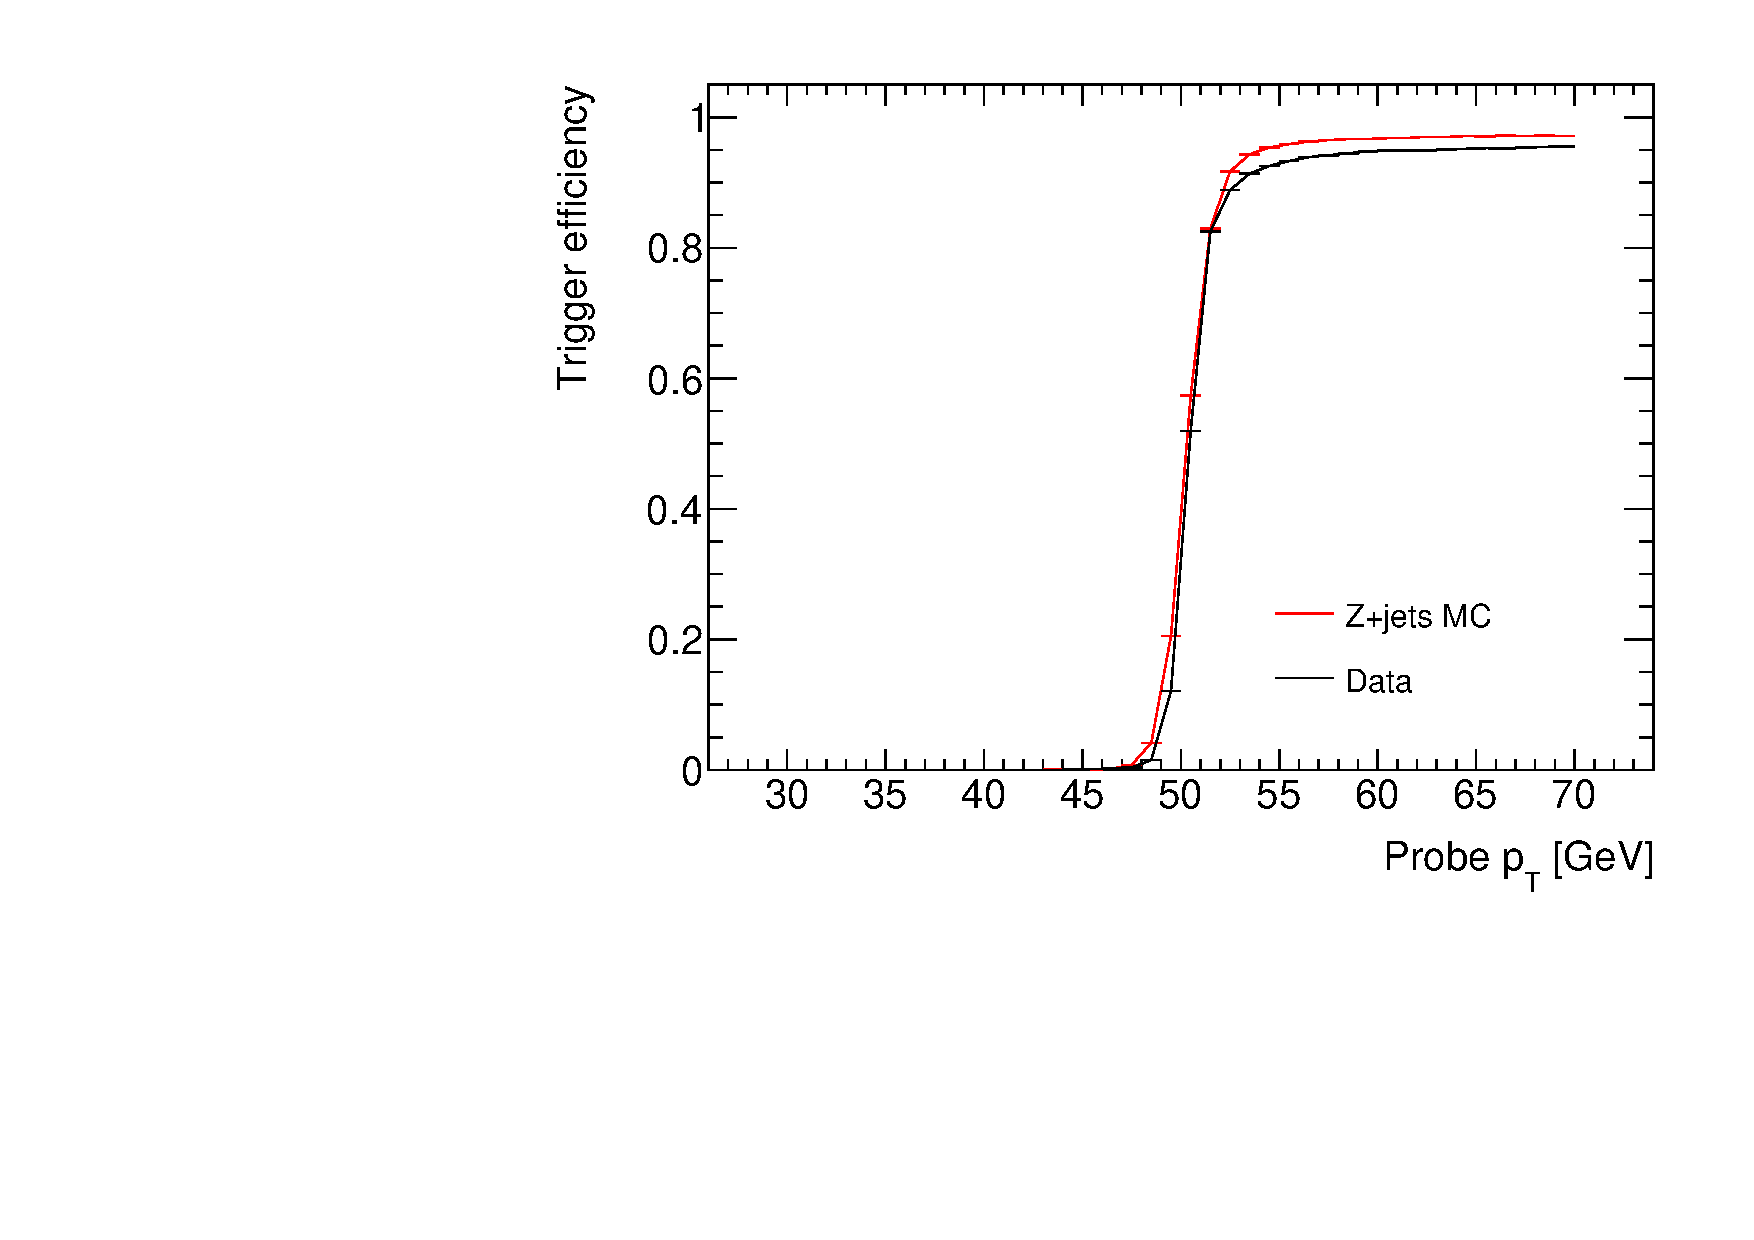
\includegraphics[width = 0.44 \textwidth]{figures/PhotonTrigEff/diph_eff_pt.pdf}}
    \subfloat[]{\label{fig:PhotonTrigEff:si_pt}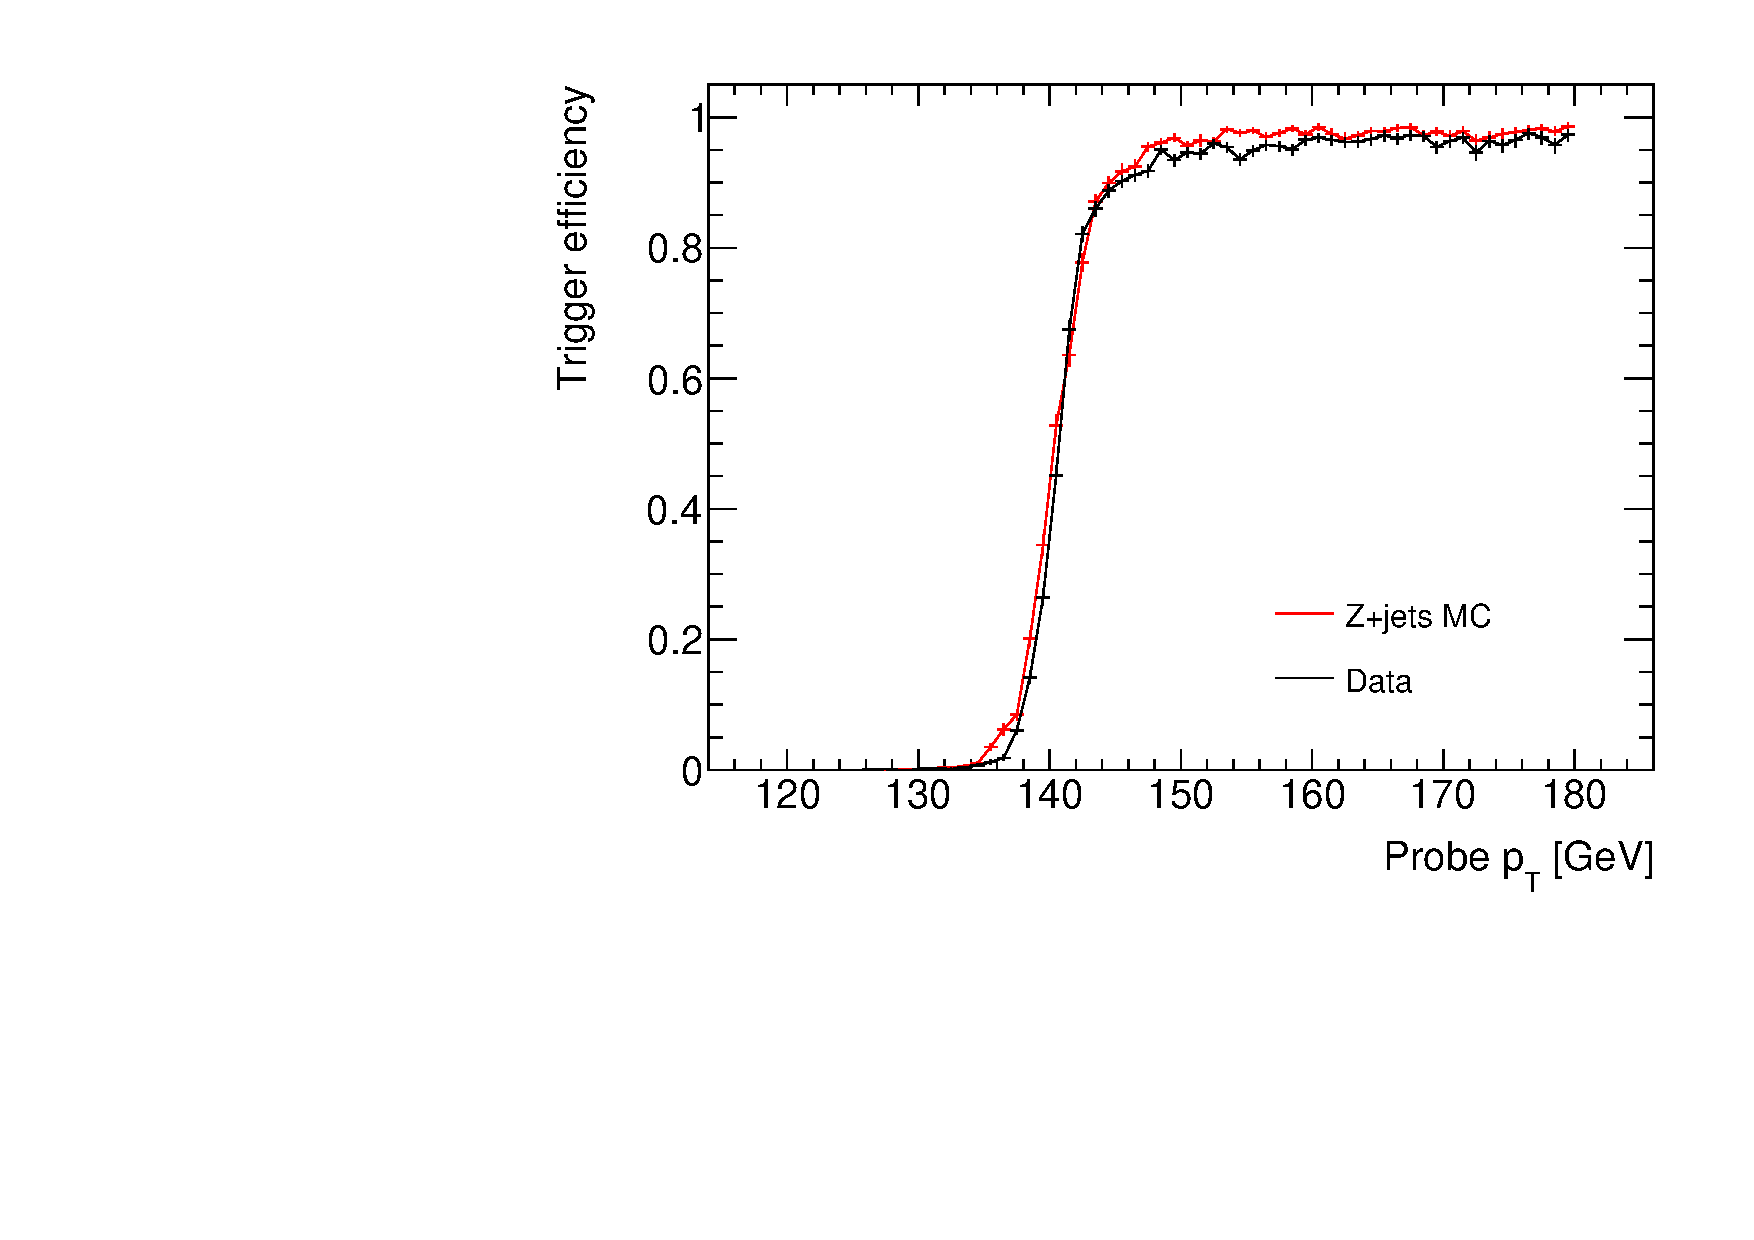
\includegraphics[width = 0.44 \textwidth]{figures/PhotonTrigEff/siph_eff_pt.pdf}} \\
    \subfloat[]{\label{fig:PhotonTrigEff:di_eta}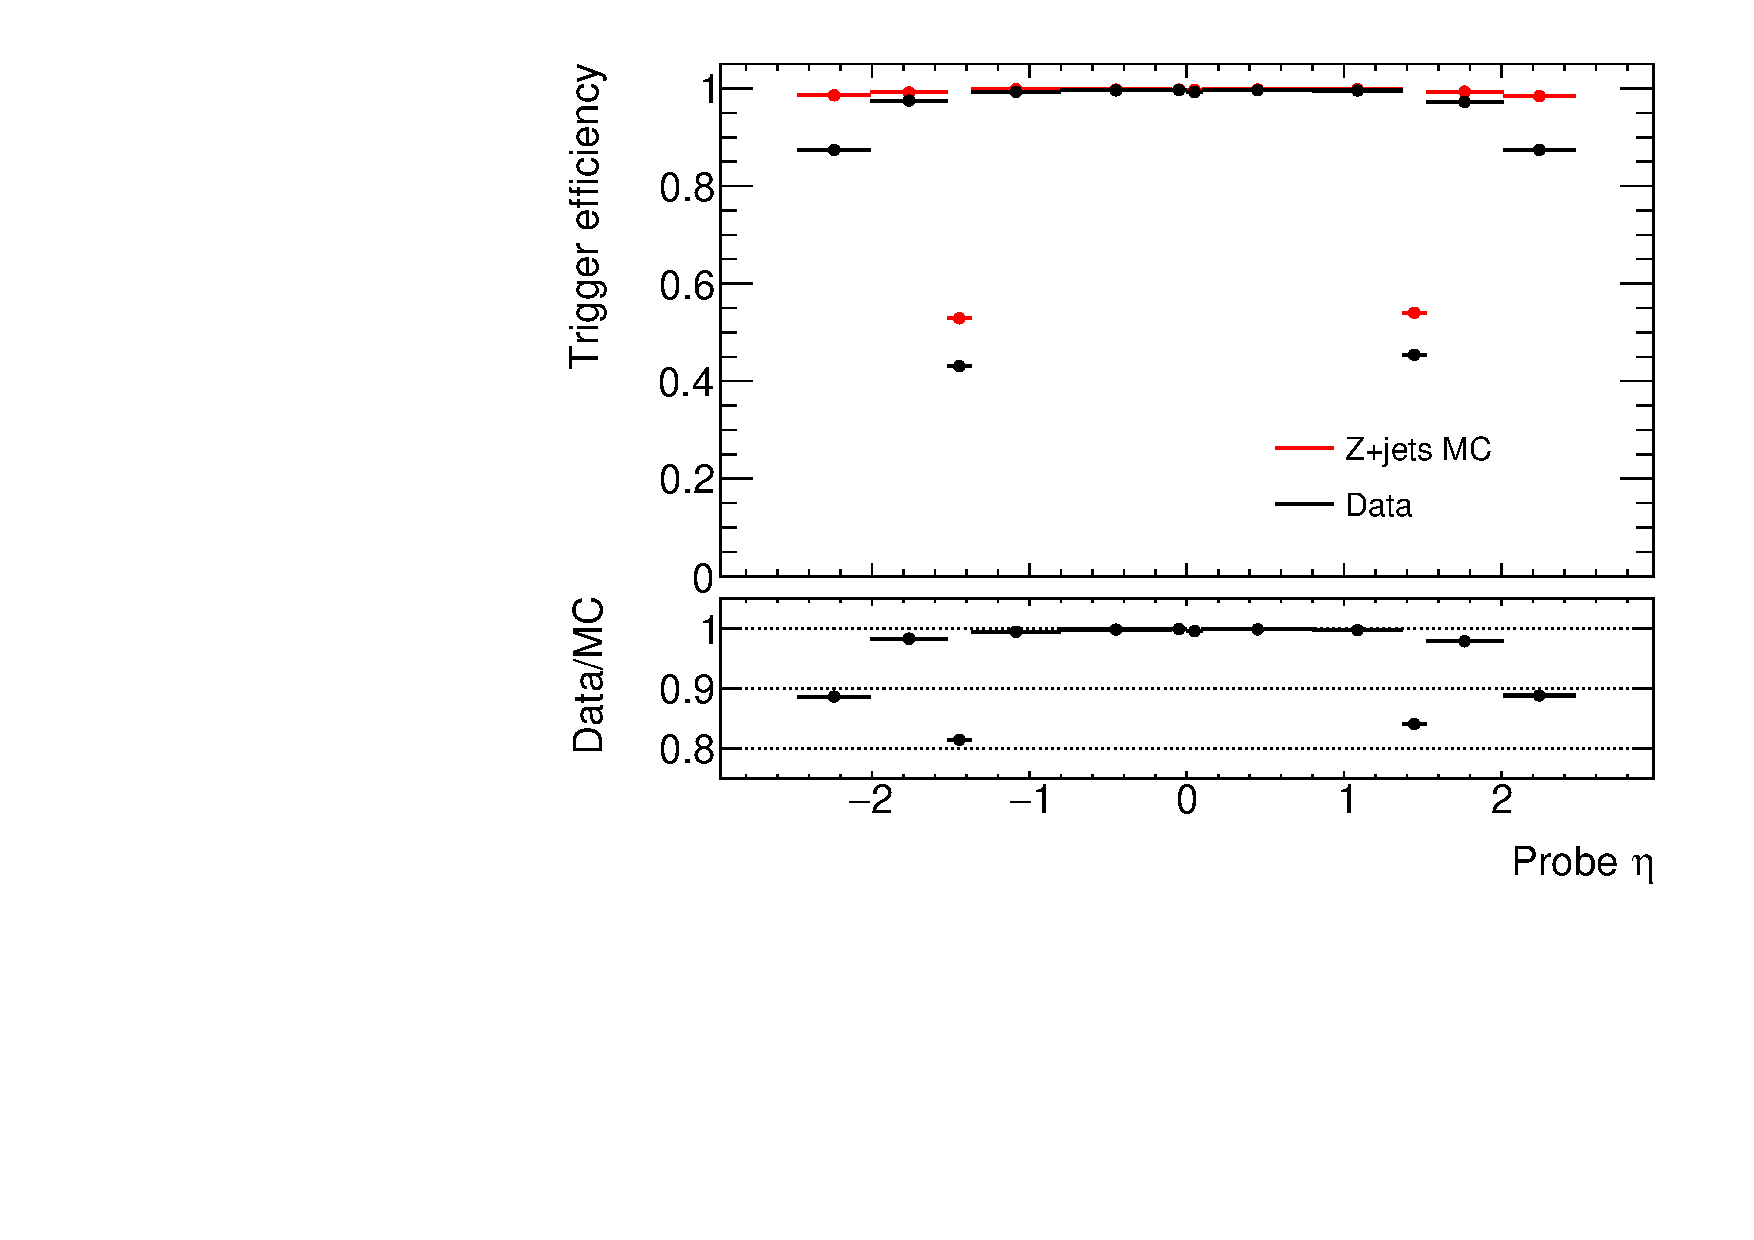
\includegraphics[width = 0.44 \textwidth]{figures/PhotonTrigEff/diph_eff_eta.pdf}}
    \subfloat[]{\label{fig:PhotonTrigEff:si_eta}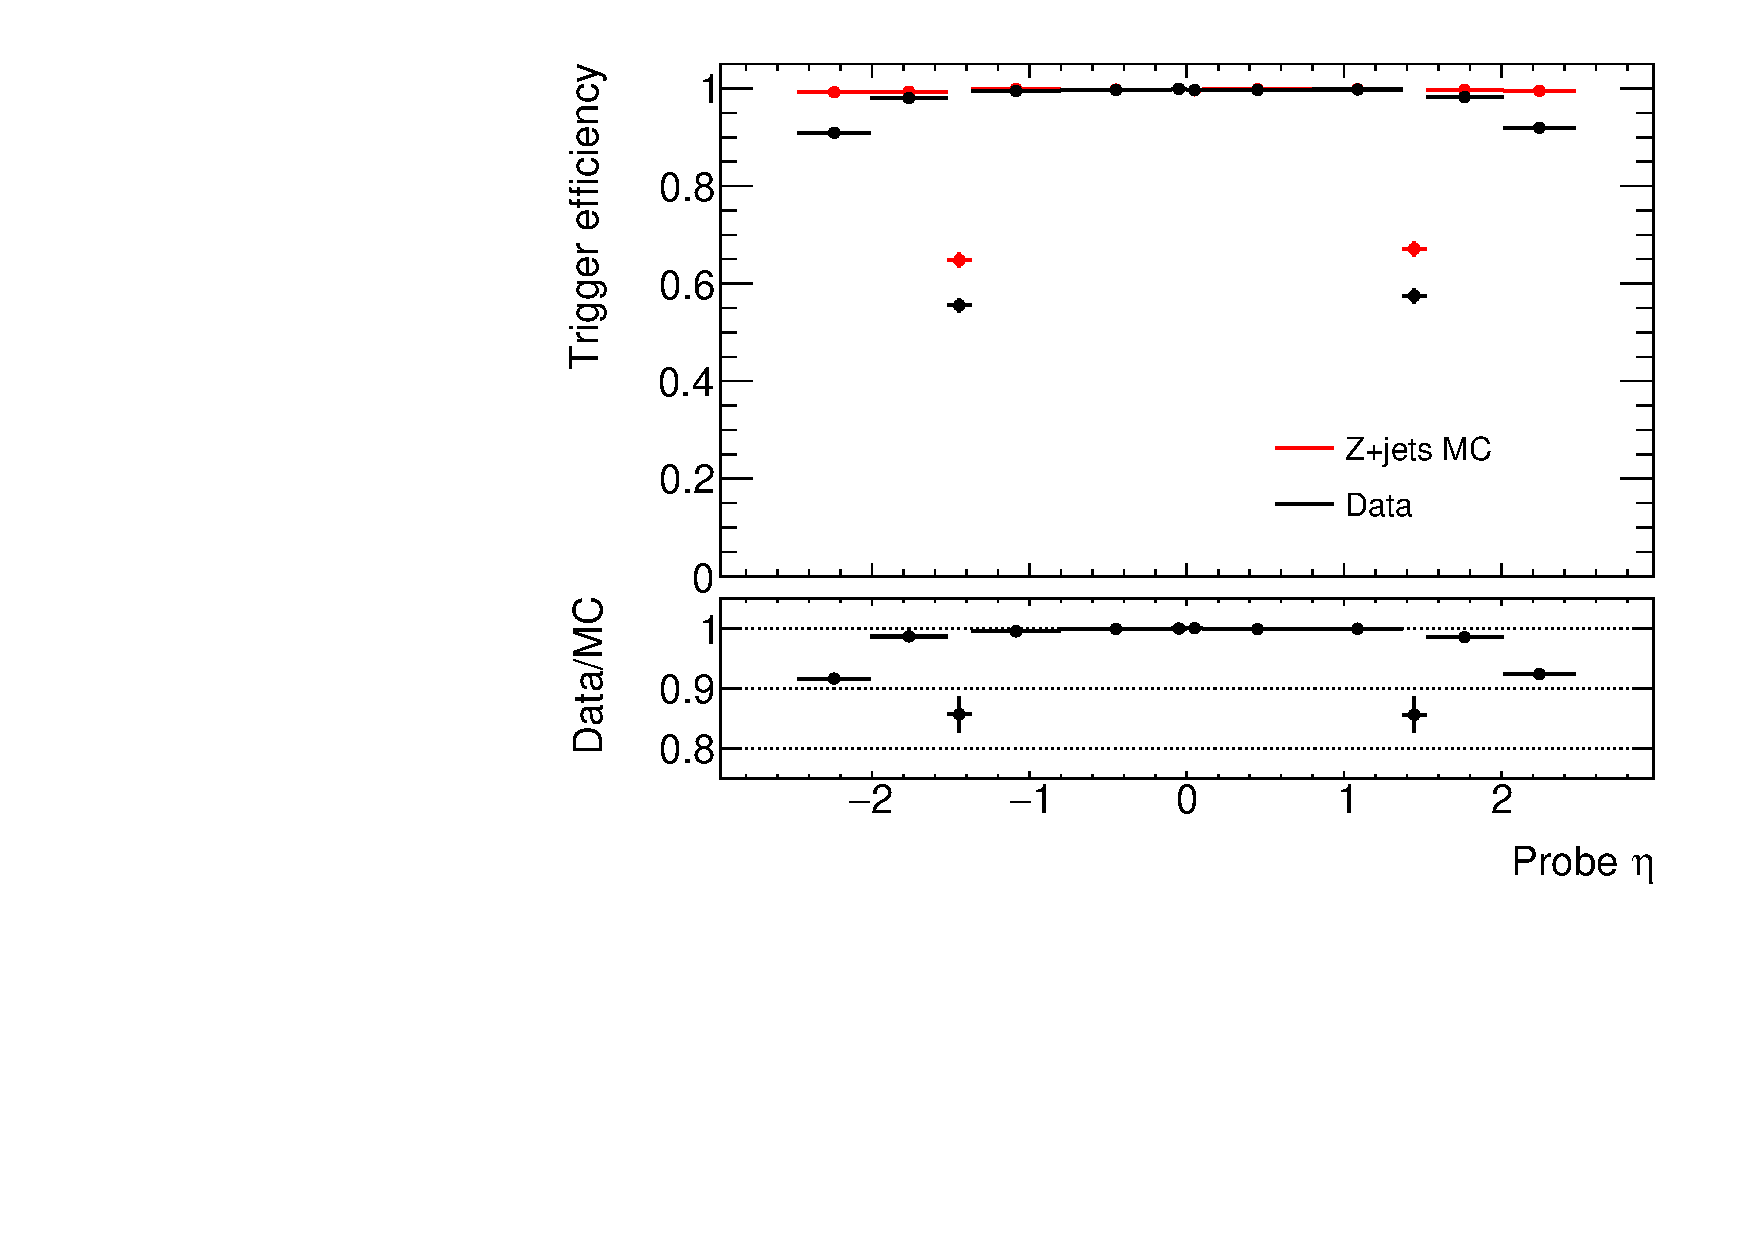
\includegraphics[width = 0.44 \textwidth]{figures/PhotonTrigEff/siph_eff_eta.pdf}} \\
    \subfloat[]{\label{fig:PhotonTrigEff:di_z0}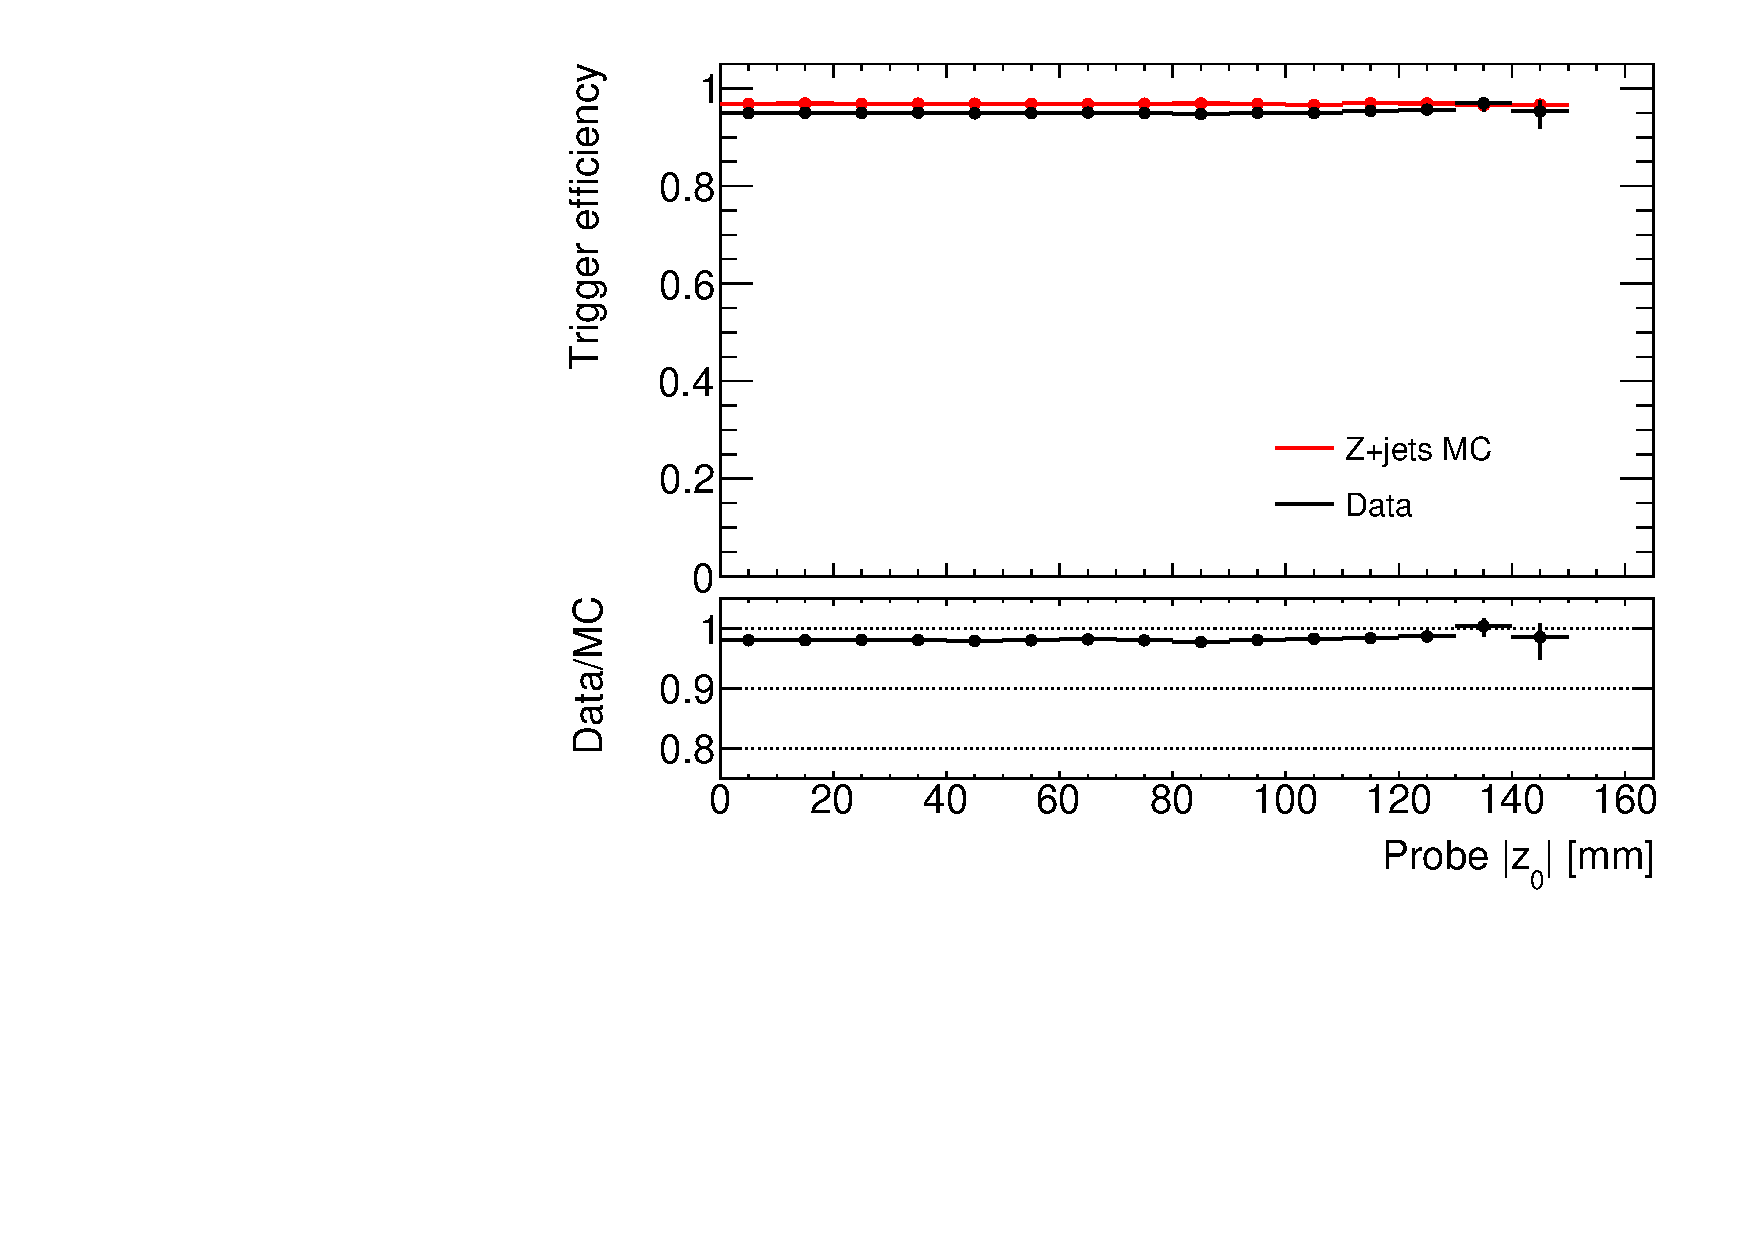
\includegraphics[width = 0.44 \textwidth]{figures/PhotonTrigEff/diph_eff_z0.pdf}}
    \subfloat[]{\label{fig:PhotonTrigEff:si_z0}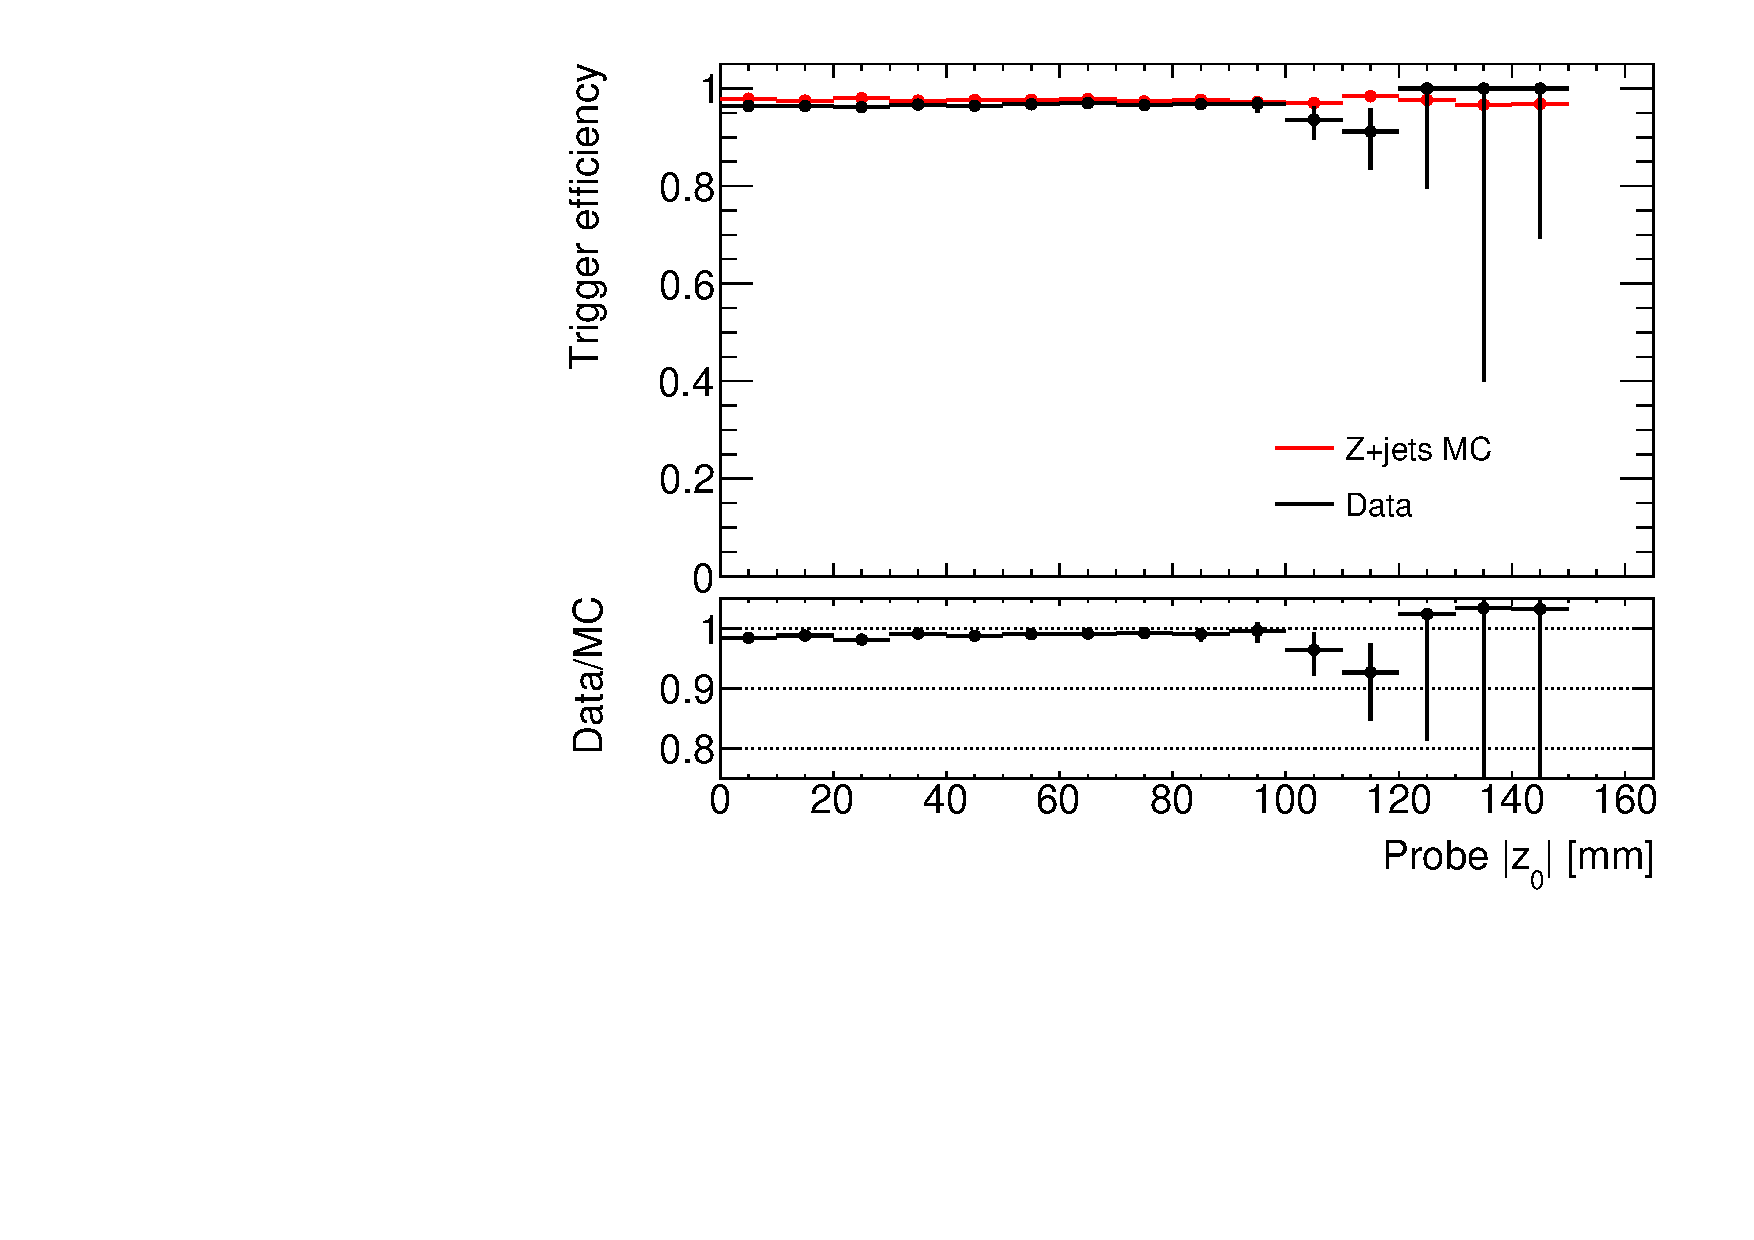
\includegraphics[width = 0.44 \textwidth]{figures/PhotonTrigEff/siph_eff_z0.pdf}}
    \caption{Efficiencies of the \texttt{HLT\_g50\_loose} as a function of probe (a) $p_{T}$, (c) $\eta$, and (e) $|\zzero|$ estimated using the data and $Z$+jets MC samples. The corresponding plots of the \texttt{HLT\_g140\_loose} trigger are shown in (b), (d), and (f). Only the pairs with a probe electron in the plateau region of (a) and (b) are considered in the rest.
    }
    \label{fig:PhotonTrigEff}
\end{figure}




\subsection{Muon trigger}
\label{subsect:muonTrigEff}

The systematic uncertainty of the single muon trigger is estimated with a standard tag-and-probe method on $Z \rightarrow \mu\mu$ events both in data and MC. The selection criteria of muon tag-and-probe candidates are listed in Table~\ref{tab:ZmmSelection}. Similar to the photon triggers, pairs are required to have opposite signs and to satisfy the mass requirement ($|m_{e^{+}e^{-}} - m_{Z}| < 10~\si{\GeV}$) and the isolation requirement of $\DeltaR(\mathrm{tag}, \mathrm{probe}) > 0.4$. 

\begin{table}[!htb]
	\centering
	\begin{tabular}{ccc}
		\hline
		\hline
		Cut & Tag muon & Probe muon \\
		\hline
		$p_{T}$ [GeV] $>$ & 28 & 30 \\
		Trigger matched & \texttt{HLT\_mu26\_ivarmedium} & --- \\
		$|\eta| <$ & 2.4 & 1.05 \\
		Identification & Medium & Loose and combined \\
		Isolation & Loose & --- \\
		\dzero significance & $< 3$ & --- \\
		$\Delta \zzero \sin{\theta}$ & $< 0.5 \si{\mm}$ & --- \\
		\hline
		\hline
	\end{tabular}
	\caption{Selection criteria for tag-and-probe muons.}
	\label{tab:ZmmSelection}
\end{table}

The invariant mass distributions of the muon tag-and-probe pairs found in the data and MC samples are shown in Figure~\ref{fig:MuonTrigMass}. The shape of distribution is in good agreement with negligible background. Therefore, no background subtraction is performed in the calculation of the trigger efficiency.

\begin{figure}[!htb]
    \centering
    \subfloat{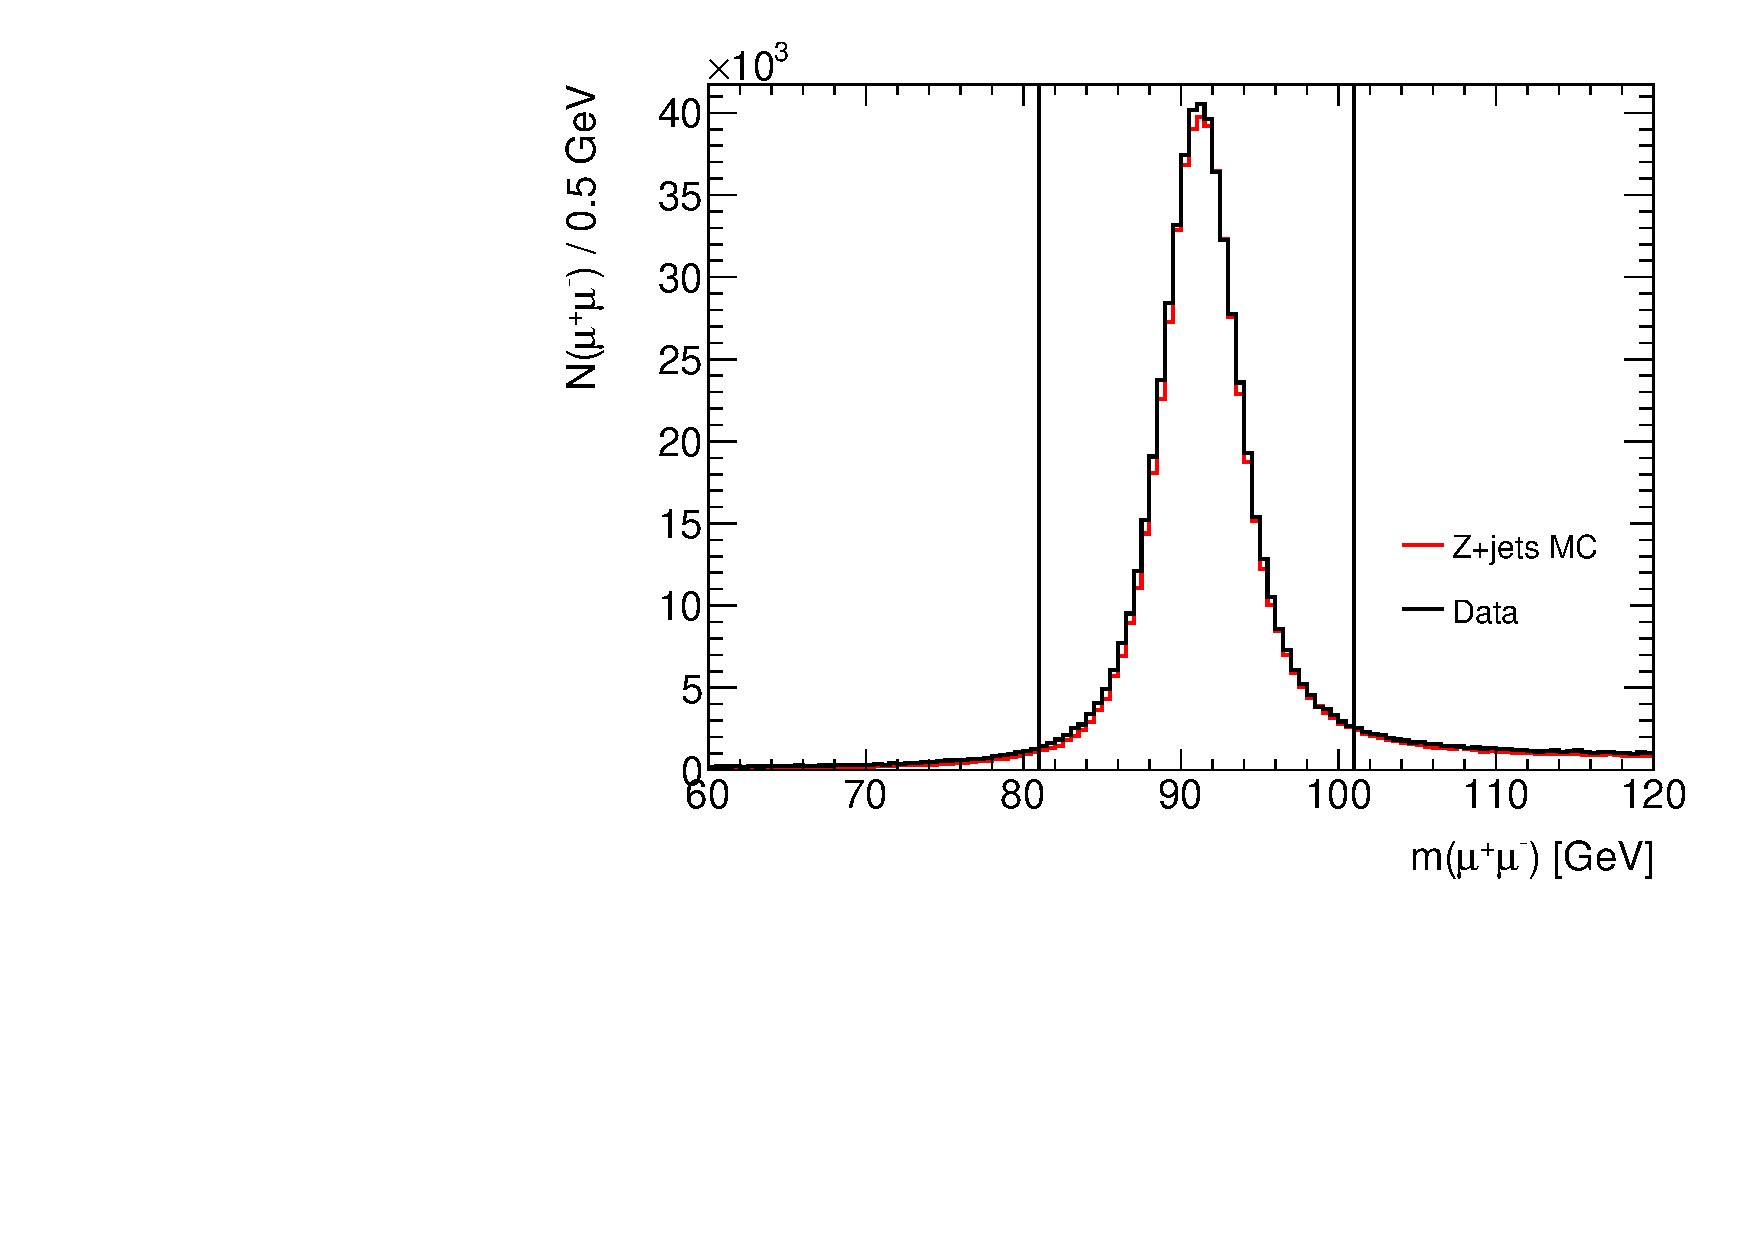
\includegraphics[width = 0.44 \textwidth]{figures/MuonTrigEff/mass.pdf}}
    \caption{Invariant mass distributions of the tag-and-probe muon pairs used to study the efficiencies of the single muon trigger in the data and $Z$+jets MC samples. Only the pairs with a probe muon in the plateau region of Figure~\ref{fig:MuonTrigEff1Da} are considered.
    }
    \label{fig:MuonTrigMass}
\end{figure}

The selected tag-and-probe muons are used to estimate the efficiency of the single muon trigger, shown as a function of probe $p_{T}$ and $|\zzero|$ in Figure~\ref{fig:MuonTrigEff1D}. The efficiency in $p_{T}$ show that the muon trigger plateau starts at $62 \si{\GeV}$. The efficiency in $|\zzero|$ shows no dependence of the muon trigger efficiency on $|\zzero|$. However, the trigger efficiency in data can be studied up to $|\zzero| \approx 150~\si{\mm}$ at which a significant decrease in the efficiency is shown.


\begin{figure}[!htb]
    \centering
    \subfloat[\label{fig:MuonTrigEff1Da}]{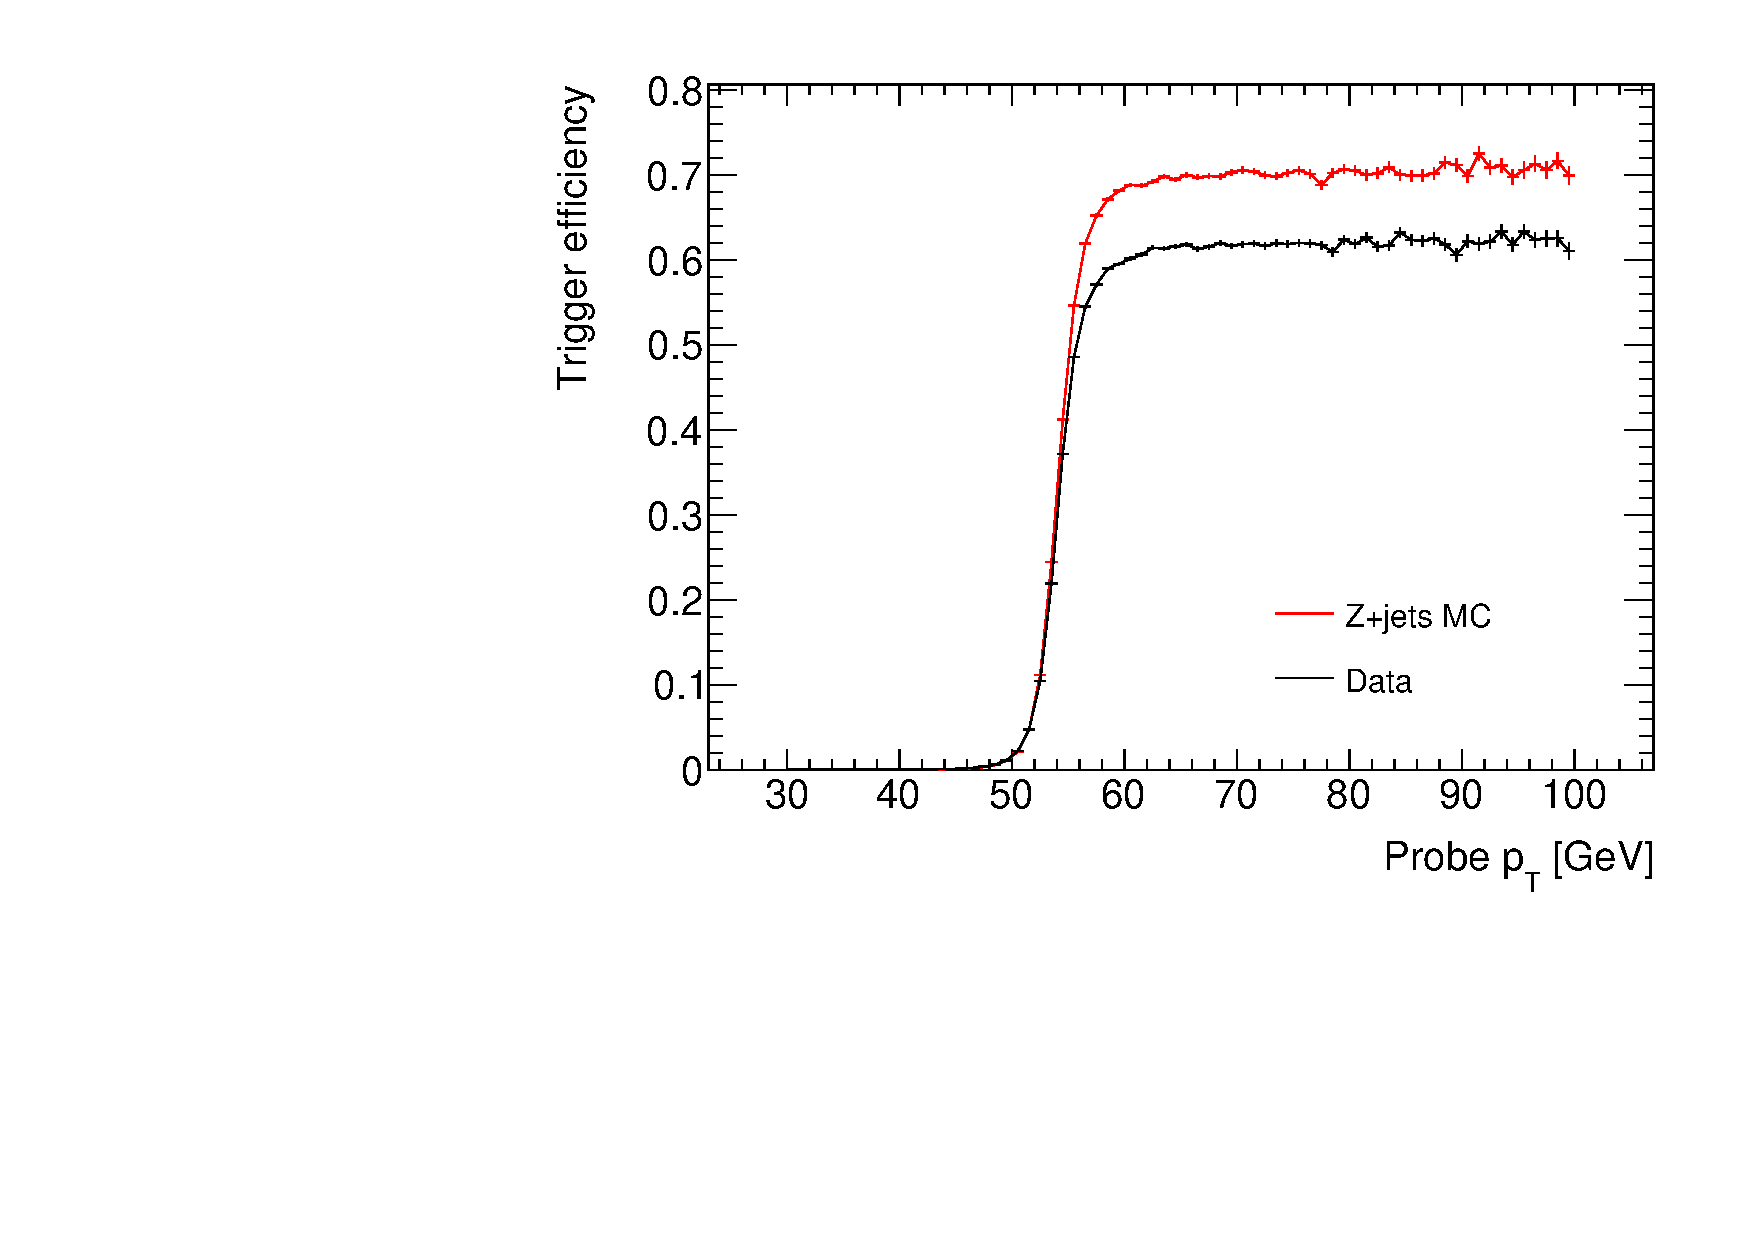
\includegraphics[width = 0.44 \textwidth]{figures/MuonTrigEff/simu_pt.pdf}}
    \subfloat[\label{fig:MuonTrigEff1Db}]{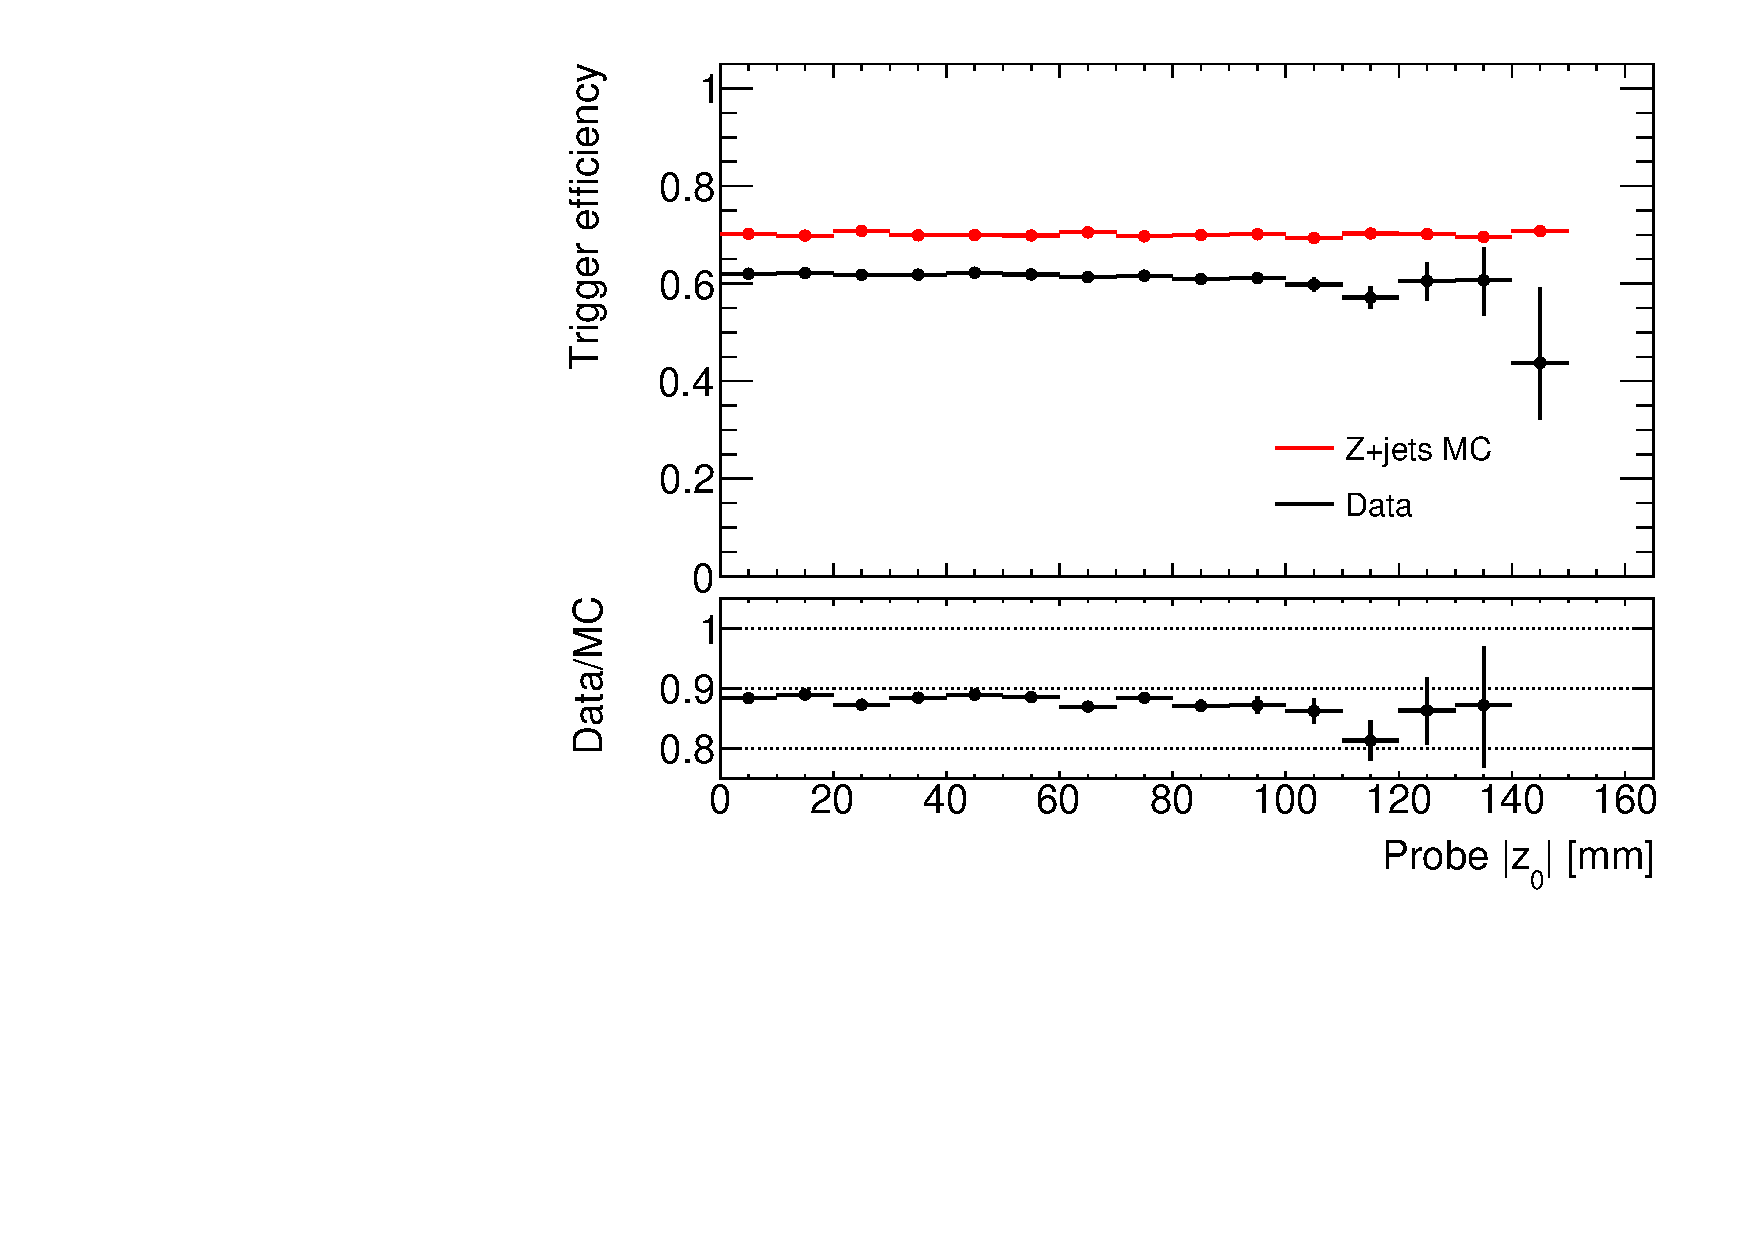
\includegraphics[width = 0.44 \textwidth]{figures/MuonTrigEff/simu_z0.pdf}}
    \caption{Efficiency of the single muon trigger as a function of probe (a) $p_{T}$ and (b) |\zzero| estimated using the data and $Z$+jets MC samples. Only the pairs with a probe electron in the plateau region of (a) are considered in (b).}
    \label{fig:MuonTrigEff1D}
\end{figure}





\begin{table}[!htb]
	\centering
	\begin{tabular}{cc}
		\hline
		\hline
		Source                              &       Syst. Uncert.       \\
		\hline
        Trigger                             &       -                   \\
        Track reconstruction                &       14\%                \\
        Vertex reconstruction               &       1\%                 \\
		\hline
        Total                               &       15\%                \\
		\hline
		\hline
	\end{tabular}
	\caption{Summary table of all systematic uncertainties in the signal efficiency}
	\label{tab:syst_total}
\end{table}


























